% -----------------------------------------------------------------
%        File: thesis.tex
% Description: Thesis
%      Author: Andrew Parlane
% -----------------------------------------------------------------

% This file is part of https://github.com/andrewparlane/fiuba_thesis
% Copyright (c) 2022 Andrew Parlane.
%
% This is free software: you can redistribute it and/or modify it under
% the terms of the GNU General Public License as published by the Free
% Software Foundation, version 3.
%
% This program is distributed in the hope that it will be useful, but
% WITHOUT ANY WARRANTY; without even the implied warranty of
% MERCHANTABILITY or FITNESS FOR A PARTICULAR PURPOSE. See the GNU
% General Public License for more details.
%
% You should have received a copy of the GNU General Public License
% along with this code. If not, see <http://www.gnu.org/licenses/>.

% Note: This thesis was written and compiled using overleaf
%       Building it via pdflatex has been tested, but not extensively

\documentclass[a4paper, twoside, 11pt]{report}

% =============================================
% Includes
% =============================================

% packages
% -----------------------------------------------------------------
%        File: packages.tex
% Description: Various packages
%      Author: Andrew Parlane
% -----------------------------------------------------------------

% This file is part of https://github.com/andrewparlane/fiuba_thesis
% Copyright (c) 2022 Andrew Parlane.
%
% This is free software: you can redistribute it and/or modify it under
% the terms of the GNU General Public License as published by the Free
% Software Foundation, version 3.
%
% This program is distributed in the hope that it will be useful, but
% WITHOUT ANY WARRANTY; without even the implied warranty of
% MERCHANTABILITY or FITNESS FOR A PARTICULAR PURPOSE. See the GNU
% General Public License for more details.
%
% You should have received a copy of the GNU General Public License
% along with this code. If not, see <http://www.gnu.org/licenses/>.

% Maths stuff (\begin{align*} for one)
\usepackage{amsmath}

% Spanish Localisation
\usepackage[spanish]{babel}

% UTF8 encoding allows for accents. Must come before biblatex
\usepackage[utf8]{inputenc}

% Bibliography
\usepackage[backend=biber, style=numeric]{biblatex}

% For \captionsetup
\usepackage{caption}

% Required by biblatex and must come after inputenc
\usepackage{csquotes}

% dirtree (for outputting the dir tree of the repos)
\usepackage{dirtree}

% Better lists, allows setting \parsep
\usepackage{enumitem}

% A4 + default margins
\usepackage[a4paper]{geometry}

% Images
\usepackage{graphicx}

% For embedding code
\usepackage{listings}

% Multirow
\usepackage{multirow}

% for \nicefrac
\usepackage{nicefrac}

% For \onehalfspacing
\usepackage{setspace}

% For \FloatBarrier
\usepackage{placeins}

% SI Units
\usepackage{siunitx}

% Allows for setting space between sections
\usepackage[compact]{titlesec}

% Links (must be loaded after titlesec)
\usepackage{hyperref}

% Fix links to images so they actually show the image
\usepackage[all]{hypcap}

% TabularY (for autosizing columns (L) in the port list tabels)
\usepackage{tabulary}

% Change spacing around ToC
\usepackage{tocloft}

% Colours for table row zebras
\usepackage[table]{xcolor}


% settings
% -----------------------------------------------------------------
%        File: settings.tex
% Description: Various configuration settings
%      Author: Andrew Parlane
% -----------------------------------------------------------------

% This file is part of https://github.com/andrewparlane/fiuba_thesis
% Copyright (c) 2022 Andrew Parlane.
%
% This is free software: you can redistribute it and/or modify it under
% the terms of the GNU General Public License as published by the Free
% Software Foundation, version 3.
%
% This program is distributed in the hope that it will be useful, but
% WITHOUT ANY WARRANTY; without even the implied warranty of
% MERCHANTABILITY or FITNESS FOR A PARTICULAR PURPOSE. See the GNU
% General Public License for more details.
%
% You should have received a copy of the GNU General Public License
% along with this code. If not, see <http://www.gnu.org/licenses/>.


% Don't indent paragraphs
\setlength{\parindent}{0cm}

% Space between paragraphs
\parskip 1.5ex

% Line spacing: 1.5
\onehalfspacing

% Reduce space between items in \begin{description}, \begin{itemize} and \begin{enumerate}
\setlist[description]{noitemsep, nolistsep, topsep=0pt}
\setlist[itemize]{noitemsep, nolistsep, topsep=0pt}
\setlist[enumerate]{noitemsep, nolistsep, topsep=0pt}

% Change Table of Contents name from "Índice General" to "Índice"
\addto\captionsspanish{
  \renewcommand{\contentsname}
    {Índice}
}

% \Chapter format - Huge, bold, no numbering
\titleformat{\chapter}{\normalfont\Huge\bfseries}{}{0pt}{}

% Reduce space before and after the \chapter title
\titlespacing{\chapter}{0pt}{-1em}{1em}

% \Section format - huge, bold
\titleformat{\section}{\normalfont\huge\bfseries}{\thesection}{0pt}{}

% \Subsection format - LARGE, bold
\titleformat{\subsection}{\normalfont\LARGE\bfseries}{\thesection}{0pt}{}

% \subsubsection format - Large
\titleformat{\subsubsection}{\normalfont\Large}{\thesection}{0pt}{}

% Don't number sections
\setcounter{secnumdepth}{0}

% Sets links to blue
\hypersetup{
    colorlinks,
    citecolor=blue,
    filecolor=blue,
    linkcolor=blue,
    urlcolor=blue
}

% ToC depth to \subsubsection
\setcounter{tocdepth}{3}

% Remove spacing at top of page before and after the Índice title
\setlength{\cftbeforetoctitleskip}{0pt}
\setlength{\cftaftertoctitleskip}{0pt}

% Don't hyphonate over pages
\brokenpenalty10000\relax

% Captions should "hang" aka align with the start, and not with the label
\captionsetup{format=hang}

% Create a new command for referencing figures with "Figura ?.?" as the link. Same for tables and sections
% Call with:
%  \figref{fig:figure-label} 
%  \tabref{tab:table-label}
%  \secref{sec:section-label}{Section Name}
\newcommand*{\figref}[1]{\hyperref[#1]{Figura~\ref*{#1}}}
\newcommand*{\tabref}[1]{\hyperref[#1]{Cuadro~\ref*{#1}}}
\newcommand*{\secref}[2]{\hyperref[#1]{Sección #2}}

% Zebra pattern in tables
\newcommand*{\tablezebra}{\rowcolors{2}{white}{lightgray!35}}

% Let's us restart the row num to reset the zebra pattern using \setcounter{rownum}{0}
\makeatletter
\@ifundefined{c@rownum}{\let\c@rownum\rownum}{}
\makeatother


% Bibliography
\addbibresource{bibliography.bib}

% =============================================
% Document
% =============================================

\begin{document}

% ---------------------------------------------
% Title Page
% ---------------------------------------------
\begin{titlepage}

\capstartfalse
\begin{figure}
\centering
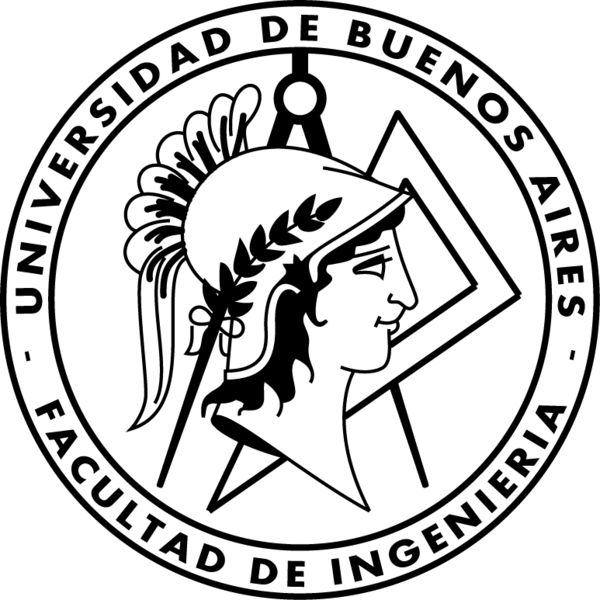
\includegraphics[scale=1.7]{./img/logo-facu.png}
\end{figure}
\capstarttrue

\begin{center}
    \Large{Universidad de Buenos Aires} \\
    \Large{Facultad de Ingeniería} \\
    \Large{Tesis de Maestría en Ciencias de la Ingeniería} \\
    \vspace{5mm}
    \huge{\bf Desarrollo de circuitos integrados CMOS para aplicaciones de RFID} \\
    \vspace{8mm}
    \huge{\bf Andrew Parlane}
\end{center}

\vspace*{\fill}

\begin{description}
    \item[\large{Director:}] \hspace{21pt} \large{Dr. Ing. Mariano Garcia-Inza}
    \item[\large{Codirectores:}] \large{Ing. Federico G. Zacchigna, Ing. Octavio Alpago}
\end{description}
\end{titlepage}

% ---------------------------------------------
% Resumen
% ---------------------------------------------

\FloatBarrier
%\chapter* so it doesn't get added to the ToC
\chapter*{Resumen}
Este trabajo presenta el diseño de circuitos integrados digitales para la implementación de un TAG RFID en un chip CMOS. Los requerimientos de los circuitos son definidos por un proyecto de investigación marco cuyo objetivo general es el desarrollo de sensores inalámbricos de radiación ionizante para dosimetría médica. Esto requiere la integración de diferentes subsistemas en un ASIC a fabricar en tecnología CMOS.

Los circuitos presentados en esta tesis consisten en un bloque digital de control, que puede recibir y responder a las tramas definidas en la norma ISO/IEC 14443A, y mediante un protocolo propietario encima de la norma, controlar otros subcircuitos del chip necesarios para la adquisición de la señal dosimétrica y su posterior transmisión inalámbrica. La implementación de la norma es presentada en un núcleo IP genérico. Por lo tanto es apto para uso en otros proyectos y con cualquier lector comercial que trabaje bajo norma. El protocolo propietario consiste en cinco mensajes que permiten el muestreo de hasta quince TAGs de forma sincronizada. El muestreo simultáneo de múltiples TAGs sensores utilizando RFID es una estrategia novedosa desarrollada en esta tesis, el cual representa un potencial avance en el desarrollo de métodos de control dosimétrico en aplicaciones médicas.

El trabajo realizado incluye el diseño de los bloques digitales utilizando HDL SystemVerilog y su verificación funcional. Luego, se utiliza el kit de diseño del proceso (PDK, por sus siglas en Inglés) XH018 (nodo tecnológico de \SI{180}{\nano\meter}) de la foundry XFAB para realizar la síntesis, el place and route y la generación de las máscaras de fabricación (layout).

Las pruebas de verificación llevadas a cabo dan alta confianza en el diseño. Las mismas incluyen: más de cien horas de simulaciones del RTL ejecutando 187 aserciones de SystemVerilog más de cien mil millones de veces y generando informes de cobertura de código, la verificación formal de equivalencia entre lógica RTL y los netlists post síntesis y post implementación, Design Rules Check (DRC), y Layout Vs Schematic (LVS); todas esas pruebas tienen resultados favorables.

El layout final no tiene violaciones de timing, el slack de Setup menor es \SI{1,59}{\nano\second} y de Hold es \SI{0,02}{\nano\second}, el área utilizada es \SI{0,087}{\milli\meter\squared} (\SI{295,68}{\micro\meter} por \SI{294,00}{\micro\meter}), y la estimación de consumo de potencia promedio es \SI{256}{\micro\watt}.

% ---------------------------------------------
% Aclaraciones
% ---------------------------------------------

\FloatBarrier
%\chapter* so it's not in the ToC
\chapter*{Aclaraciones}

Aclaraciones
Por cuestiones de claridad en esta tesis cuándo se dice que una señal está en ‘1’ o ‘0’ significa que la señal tiene un valor lógico igual a '1' o ‘0’ respectivamente.

El código RTL, los bancos de pruebas y los scripts de síntesis y place \& route están publicados de forma abierta en GitHub bajo la licencia GNU v3.0, de manera que cualquier parte de este trabajo pueda ser utilizada en otros proyectos académicos o comerciales. Para facilitar la adopción y modificación de este trabajo por la comunidad internacional, el código y los scripts están escritos con nombres y comentarios en Inglés.

Para facilitar la lectura de esta tesis las señales, variables y parámetros están escritos en \textit{cursiva},  los módulos, clases y funciones están escritos en \textbf{negritas}. Además se utilizan paréntesis para nombrar a las funciones, aunque sin sus argumentos, por ejemplo: \textbf{compare()}. Finalmente los nombres de las tramas definidas en los protocolos están escritos en MAYÚSCULAS.

% ---------------------------------------------
% TOC
% ---------------------------------------------
\newpage
\tableofcontents

% ---------------------------------------------
% Introducción
% ---------------------------------------------

\FloatBarrier
\chapter{Introducción}

% Motivación y Contexto de Trabajo
% --------------------------------
\FloatBarrier
\section{Motivación y Contexto de Trabajo}

La radioterapia es un tratamiento médico que consiste en utilizar radiación ionizante para eliminar células cancerígenas que forman tumores. Sin embargo, la radiación puede presentar riesgos a tejido sano, especialmente si la dosis aplicada es mayor a la necesaria o mal localizada. Hay varios incidentes registrados donde algunas personas recibieron una sobredosis durante radioterapia, y en algunos casos dosis letales~\cite{UNSE_2019}. Por otro lado, una dosis localizada pero demasiado pequeña reduciría la efectividad del tratamiento. Por esas razones es muy importante adoptar consideraciones de QA (Quality Assurance), la cual puede definirse como:

\begin{displaycquote}[traducción mía]{qa_in_radiotherapy}
Los procedimientos que aseguren el cumplimiento de las prescripciones médicas con respeto a la dosis entregada al volumen deseado, junto con una dosis mínima a tejido sano, exposición mínima al personal, y el monitoreo adecuado del paciente para determinar el resultado del tratamiento.
\end{displaycquote}

Una técnica importante en QA es dosimetría in-vivo (IVD), que es la práctica de medir la dosis recibida durante el tratamiento en tiempo real. La IVD es recomendada para su uso en radioterapia~\cite{AAPM-1994}\cite{ICRP-2000}, con un error menor del 3\% por tratamiento. Existen varios tipos de sensores de radiación que pueden ser utilizados en IVD con radioterapia. Entre ellos se encuentran los sensores MOSFET, los cuales tienen varias ventajas, como por ejemplo que pueden ser leídos en tiempo real o posteriormente, son pequeños y robustos, pero también tienen algunas limitaciones~\cite{UNSE_2019}. Los investigadores del Laboratorio de Física de Dispositivos - Microelectrónica de la Facultad de Ingeniería de la Universidad de Buenos Aires han trabajando durante los últimos años en mejorar el desempeño de sensores MOSFET de radiación para uso en IVD~\cite{mosfet_mismatch_amplification}\cite{6MV_LINAC}. Otra ventaja de los sensores MOSFETs es que pueden ser integrados en un mismo chip con circuitos adicionales que permitan su lectura, digitalización y posterior transmisión de los resultados en tiempo real. Esto representa una importante ventaja frente al método usual de lectura post irradiación, ya que el seguimiento en tiempo real permitiría ajustar la dosis durante la ejecución del tratamiento.

Un sensor pequeño construido con una cantidad mínima de componentes permitiría obtener arreglos de sensores con excelente resolución espacial y así realizar un mapeo dosimétrico de una zona de interés. A la hora de implementar esta solución, los TAGs RFID (Radio Frequency Identification) pasivos son una excelente opción, ya que sólo requieren del circuito integrado y una antena externa. La alimentación y la comunicación pueden realizarse a través del campo electromagnético generado por el dispositivo de lectura. Un sistema de estas características, además de ser más simple, sería más cómodo para el paciente y más práctico para su uso en el campo médico.

En su tesis de 2018~\cite{Arana_thesis}, Arana analizó la relación entre la frecuencia de operación de un TAG RFID y su distancia máxima de la lectura considerando los límites de exposición de humanos a campos electromagnéticos definidos en IEEE C95.1. Los resultados muestran que una frecuencia en el orden de 10 MHz daría el mejor rango de operación mientras manteniendo el campo electromagnético (EM) dentro de límites seguros. Esta frecuencia se encuentra cercana a los 13.56 MHz de RFID HF (High Frequency). Arana muestra en su tesis el diseño de la antena y de circuitos integrados analógicos para un TAG ISO/IEC 14443 tipo A que puede funcionar a una distancia de 30 cm de la lectura. También en una publicación de 2014~\cite{fabricio_eamta}, Alcalde et al. presentan el diseño y fabricación de un TAG RFID que implementa parte de la norma ISO/IEC 14443 tipo A. El funcionamiento es verificado a través de mediciones experimentales del sistema funcionando en loopback.

Un atributo del protocolo ISO/IEC 14443A es que permite hasta 15 TAGs activos al mismo tiempo. Esto da la posibilidad de obtener muestras de los sensores de forma sincronizada, con la ventaja de medir en múltiples lugares del cuerpo del paciente. Esto contribuye a mejorar la verificación de la ejecución del tratamiento planificado y por lo tanto se alinea con los criterios de QA.

En un artículo publicado en 2016~\cite{monolithic_180nm}, Villani et al. se desarrolló un sensor de radiación inalámbrico para uso en IVD por radioterapia. El sensor emite una señal RF con frecuencia que depende de la dosis de radiación recibida. La ventaja de este enfoque es la simplicidad del diseño, el circuito integrado no necesita un bloque digital complejo para soportar el protocolo. Las desventajas son: solo es posible usar solo un sensor a la vez, requiere una fuente de alimentación externa (batería), no permite configurar el sensor inalámbricamente, y por no haber sido diseñado dentro de una norma, no es compatible con otros equipos requiriendo de un lector diseñado ad hoc para la aplicación.

Los circuitos diseñados en esta tesis permitirán implementar una red de sensores inalámbricos cuya finalidad es medir dosis de radiación en un tratamiento de radioterapia en diferentes lugares de interés. La adquisición en múltiples puntos tiene como objetivo mejorar el control de la irradiación para ajustar con mayor precisión la dosis entregada por el acelerador a la planificación previa. Típicamente, la dosis entregada por los LINAC no es lineal con el tiempo por lo cual, para que la medición en tiempo real sea útil, se requiere sincronizar el muestreo de los sensores.

% ISO/IEC 14443A
% --------------------------------
\FloatBarrier
\section{ISO/IEC 14443A}

La norma ISO/IEC 14443 fue desarrollada por la Organización Internacional de Normalización (ISO) y la Comisión Electrotécnica Internacional (IEC), específicamente por el grupo de tareas 2 del grupo de trabajo 8 de la subcomisión del comité técnico mixto 1. Fue publicado primero en 2001 con dos interfaces distintas: tipos A y B. Tipo A fue desarrollado en colaboración con Mikron (adquirida desde entonces por Phillips), basado en su tecnología Mifare. Esta interfaz fue diseñada como una tarjeta para almacenar datos únicamente. Tipo B fue desarrollado en colaboración con varios operadores de sistemas de transporte públicos de Europa e Innovatron. Principalmente diseñado para pagos de tarifas pero también puede funcionar como billetera electrónica y verificación de identidad. Esta interfaz fue diseñada como una tarjeta que al tener un microprocesador, además de almacenar datos, cuenta con capacidad de procesamiento. Al principio estas dos interfaces fueron complementarias, pero luego de los años sus aplicaciones se ampliaron y diversificaron~\cite{14443_a_vs_b}.

La norma viene en cuatro partes:

\begin{itemize}
    \item ISO/IEC 14443-1: Características Físicas.
    \item ISO/IEC 14443-2: Radiofrecuencia Potencia y Señal Interfaz.
    \item ISO/IEC 14443-3: Inicialización y Anticolisión.
    \item ISO/IEC 14443-4: Protocolo de Transmisión.
\end{itemize}

La parte una define atributos físicas de la PICC (Proximity Card, la tarjeta o TAG) como las dimensiones y el rango de operación a temperatura ambiente. La parte dos define la interfaz inalámbrica de la transmisión de potencia y comunicaciones bidireccionales entre un PCD (Proximity Coupling Device, la lectura) y la PICC. La parte tres define el formato de los bytes, la estructura de las tramas y los mensajes necesarios para el descubrimiento de todas las PICCs presentes en el campo del PCD y para activarlas. Finalmente, la parte cuatro define un protocolo de bloques para la configuración de la PICC y la transmisión de mensajes de nivel aplicación.

Un sistema tiene un PCD que es el maestro y una o más PICCs que son los esclavas. Una PICC solo responde a solicitudes, no inicia comunicaciones. Durante el proceso de inicialización múltiples PICCs pueden responder a la misma solicitud, así colisiones son posibles y esperadas. Después del proceso de inicialización, en un sistema correctamente configurado, solo una PICC responde a cada solicitud.

\FloatBarrier
\subsection{ISO/IEC 14443-1: \large{Características Físicas}}

\message{TODO}

\FloatBarrier
\subsection{ISO/IEC 14443-2: \large{Radiofrecuencia Potencia y Señal Interfaz}}

El PCD emite un campo electromagnético con frecuencia $f_c = \SI{13.56}{\mega\hertz}$. Las PICCs dentro de este campo se acoplan inductivamente al campo para la transferencia de potencia. El campo es modulado para la comunicación entre los dispositivos. El PCD usa modulación de amplitud para enviar información a las PICCs, y las PICC envían sus respuestas con modulación de carga mediante un subcarrier. La norma define varias tasas de bits, pero las comunicaciones siempre comienzan con tasa de bits $\nicefrac{f_c}{128} \approx \SI{106}{Kbps}$ en las dos direcciones. La codificación de los bits y los parámetros de modulación dependen de: la dirección de la comunicación, si las PICCs son tipo A o B, y la tasa de bits. La \figref{fig:mod-encode} muestra una representación de las dos direcciones de comunicación para PICCs de tipo A y de tipo B.

\begin{figure}[htb]
\centering
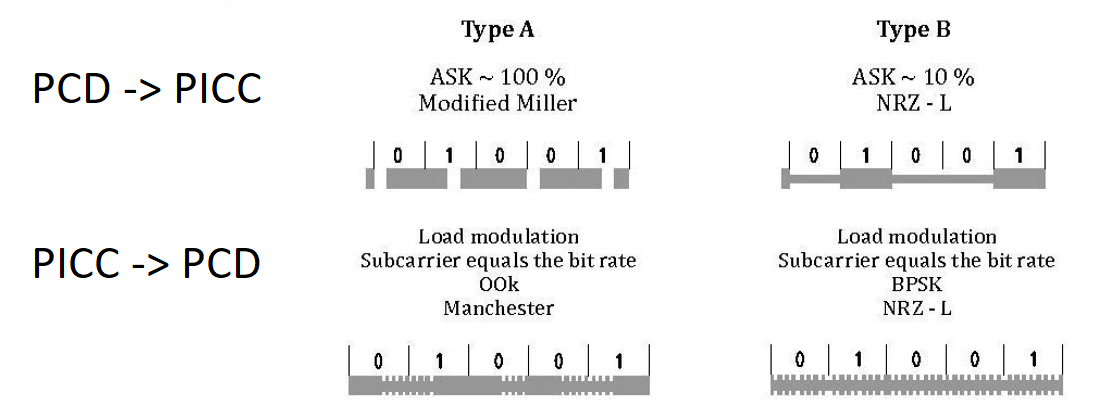
\includegraphics[scale=0.47]{./img/modulation_and_bit_encoding}
\caption{Comunicaciones con una tasa de bits de $\nicefrac{f_c}{128}$~\cite[Modificaciones Mías]{iso14443-2}}
\label{fig:mod-encode}
\end{figure}

Para PICCs de tipo A la modulación por comunicaciones desde el PCD hasta la PICC es ASK (Amplitude Shift Keying). Cuándo la amplitud de la portadora baja al 5\% del campo original, la norma define esto como una pausa. Un esquema de la misma se muestra en la \figref{fig:pause}, con valores que se definen en el \tabref{tab:pause_values}. Debido a que una PICC pasiva recibe su potencia inalámbricamente desde el campo electromagnético, es responsabilidad de la PICC mantener los rails de alimentación internos a tensiones adecuadas durante las pausas para que el sistema no cambie de estado. La codificación de los bits es Modified Miller. Cada trama comienza con un SOC (Start of Communication), tiene un número de bits de datos y termina con un EOC (End Of Communications). SOC, EOC y los valores lógicos son enviados mediante secuencias. Cada secuencia tiene el largo de una duración de bit, lo que es 128 ciclos de la portadora. La presencia y la ubicación de una pausa dentro de una duración de bit define el tipo de la secuencia, como es mostrado en la \figref{fig:sequences}. Una pausa que ocurre al principio de la duración de bit es una secuencia Z, una pausa que ocurre en el medio de la duración de bit es una secuencia X, y una bit sin pausas es una secuencia Y. El SOC es la secuencia Z. Un ‘1’ lógico es una X. Un ‘0’ lógico depende en la última secuencia, si fue una X, se envía una Y, si fue una Y o una Z, se envía una Z. La trama termina con el EOC lo que es un ‘0’ lógico, seguido por una secuencia Y. La \figref{fig:rx_frame_examples} muestra dos ejemplos de tramas.

\begin{figure}[htb]
  \centering
  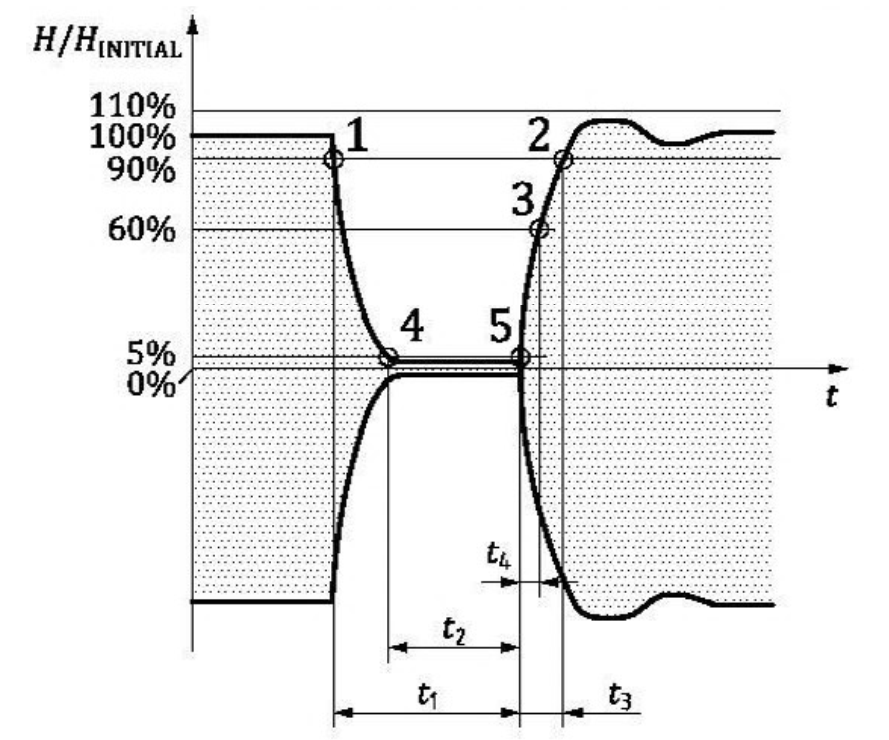
\includegraphics[scale=0.6]{./img/pause}
  \caption{El formato de una pausa tipo A~\cite{iso14443-2}}
  \label{fig:pause}
\end{figure}

\begin{table}[htb]
\centering
\begin{tabular}{|c|c|c|c|}
  \hline
  \textbf{Parámetro} & \textbf{Condición} & \textbf{Mínimo} & \textbf{Máximo} \\
  \hline
  $t_1$                   &                               & $\nicefrac{28}{f_c}$  & $\nicefrac{40,5}{f_c}$    \\
  \multirow{2}{*}{$t_2$}  & $t_1 > \nicefrac{34}{f_c}$  & $\nicefrac{7}{f_c}$   & \multirow{2}{*}{$t_1$}    \\
                          & $t_1 \le \nicefrac{34}{f_c}$  & $\nicefrac{10}{f_c}$  &                           \\
  $t_3$                   &                               & $1,5 \cdot t_4$           & $\nicefrac{16}{f_c}$      \\
  $t_4$                   &                               & 0                     & $\nicefrac{6}{f_c}$       \\
  \hline
\end{tabular}
\caption{Parámetros de timing para una pausa~\cite{iso14443-2}}
\label{tab:pause_values}
\end{table}

\begin{figure}[htb]
  \centering
  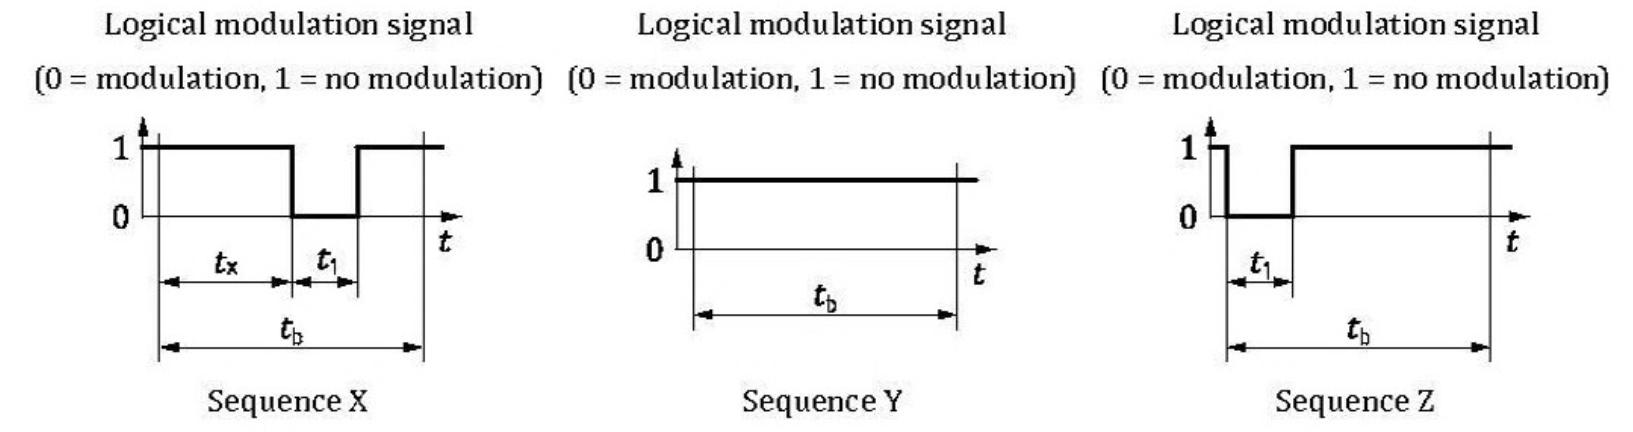
\includegraphics[scale=0.5]{./img/sequences}
  \caption{Codificación Modified Miller~\cite{iso14443-2}}
  \label{fig:sequences}
\end{figure}

\begin{figure}[htb]
  \centering
  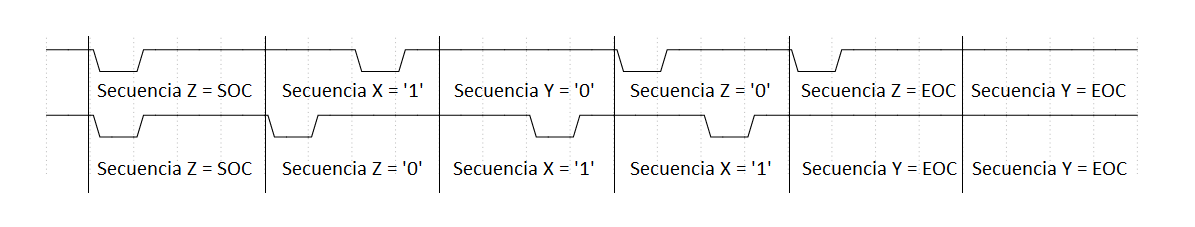
\includegraphics[scale=0.45]{./img/rx_frame_examples}
  \caption{Ejemplos de tramas PCD $\rightarrow$ PICC tipo A}
  \label{fig:rx_frame_examples}
\end{figure}

% There's a lot of images around here, make sure we keep them separated correctly
\FloatBarrier

Para responder las PICCs tipo A usan modulación de carga para generar una subportadora.  La frecuencia de la subportadora ($f_s$) depende de la tasa de bit. Para una tasa de bit de $\nicefrac{f_c}{128}$ la frecuencia es $\nicefrac{f_c}{16} \approx \SI{848}{\kilo\hertz}$. Como en el caso de comunicaciones del PCD a la PICC la duración de un bit es $\nicefrac{128}{f_c} = \nicefrac{8}{f_s}$. La portadora debe ser solo modulada con la subportadora cuando la PICC está enviando datos. Los bits a transmitir tienen codificación Manchester, para representar un ‘1’ lógico la señal es en ‘1’ por la primera mitad de la duración de bit, y en ‘0’ por la segunda mitad, para representar un ‘0’ lógico es al revés. La señal que maneja el modulador de carga es la operación lógica AND entre la señal de codificación Manchester y la subportadora como se muestra en la \figref{fig:picc_to_pcd}. Una trama comienza con un SOC lo que es un ‘1’ lógico, y termina con un EOC lo que es una duración de bit sin modulación, eso es a decir que la señal al modulador de carga es en ‘0’ por toda la duración de bit. La \figref{fig:tx_frame_example} muestra un ejemplo de una trama que ingresa a la compuerta AND con la subportadora.

\begin{figure}[htb]
  \centering
  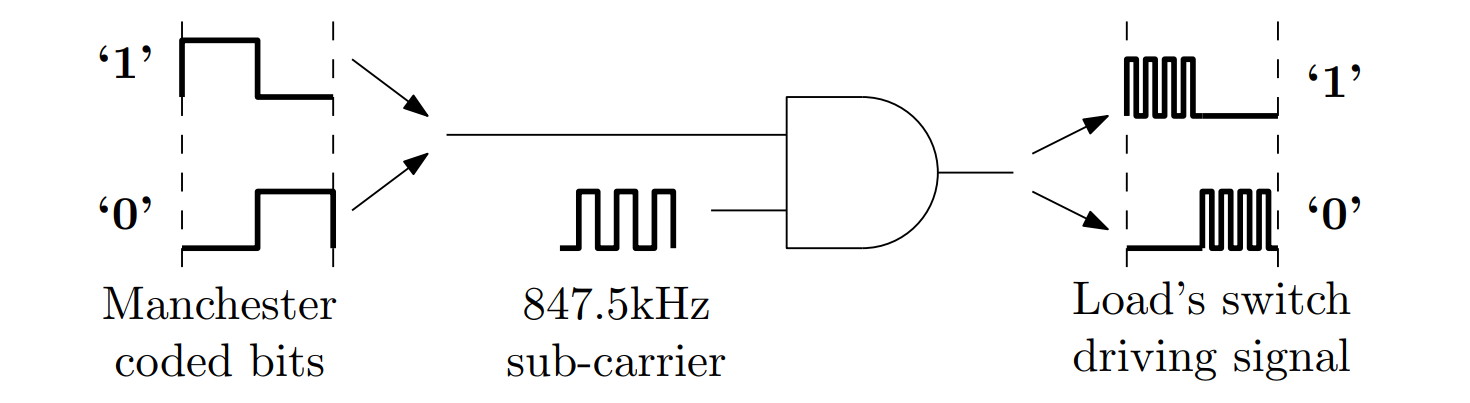
\includegraphics[scale=0.35]{./img/picc_to_pcd}
  \caption{Codificación de bits y modulación de la portadora con la subportadora para comunicaciones de la PICC a PCD~\cite{fabricio_eamta}}
  \label{fig:picc_to_pcd}
\end{figure}

\begin{figure}[htb]
  \centering
  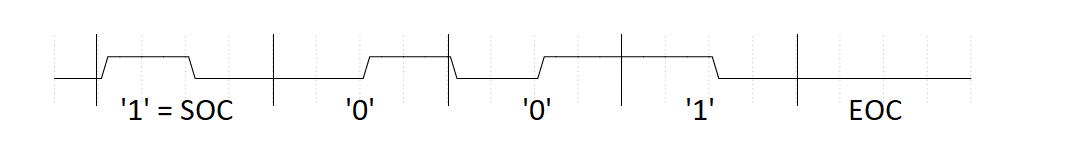
\includegraphics[scale=0.5]{./img/tx_frame_example}
  \caption{Ejemplo de una trama por comunicaciones PICC tipo A $\rightarrow$ PCD.}
  \label{fig:tx_frame_example}
\end{figure}

\FloatBarrier
\subsection{ISO/IEC 14443-3: \large{Inicialización y Anticolisión}}

La información presentada en esta sección es válida considerando una tasa de bit de fc/128 en cada dirección y PICCs tipo A.

La parte 3 de la norma define un FDT (Frame Delay Time), lo que es el tiempo entre dos tramas transmitidas en direcciones opuestas. Los tiempos del FDT definidos en la norma son especificados en números de ciclos de la portadora, y son medidos entre el último flanco de modulación de la primera trama y el primer flanco de modulación de la segunda trama. El \tabref{tab:fdt} muestra los FDTs especificados en la norma. En el caso del FDT entre una trama del PCD y una de la PICC, el FDT usado depende en el último bit lógico de la trama, y los valores especificados son absolutos para tramas de inicialización y tiempos mínimos para otras tramas.

\begin{table}[htb]
  \centering
  \begin{tabular}{|c|c|c|c|}
    \hline
    \textbf{Primera Trama} & \textbf{Segunda Trama} & \textbf{Último Bit} & \textbf{FDT} \\
    \hline
    \multirow{2}{*}{PCD~$\rightarrow$~PICC} & \multirow{2}{*}{PICC~$\rightarrow$~PCD} & '0' & 1172  \\
    \cline{3-4}
    & & '1' & 1236 \\
    \hline
    PICC~$\rightarrow$~PCD & PCD~$\rightarrow$~PICC & & 1272 \\
    \hline
  \end{tabular}
  \caption{Valores del FDT en número de ciclos de la portadora.}
  \label{tab:fdt}
\end{table}

Una trama comienza con un SOC, después se envían los datos empezando por el bit menos significativo, y termina con un EOC. Cada 8 bits de data hay un bit de paridad impar, así que el número de los 1s en cada byte más su bit de paridad es impar. Hay tres tipos de tramas definidas:

\begin{description}
  \item [Tramas Cortas] \hfill \\ Tienen siete bits de datos sin bit de paridad.
  \item[Tramas Estándares] \hfill \\ Tienen un número de bytes enteros, cada uno con un bit de paridad.
  \item[Tramas Anticolisión orientada a bits] \hfill \\ Tienen siete bytes cada uno con un bit de paridad, y están divididas en dos: la primera parte es enviada desde el PCD y la segunda parte desde la PICC. La partición puede ser después de un byte entero, incluyendo su bit de paridad (\figref{fig:anticollision} arriba), o en medio de un byte (\figref{fig:anticollision} abajo). Estas tramas son usadas durante el proceso de inicialización para que el PCD pueda detectar todas las PICCs en su campo electromagnético.
\end{description}

\begin{figure}[htb]
  \centering
  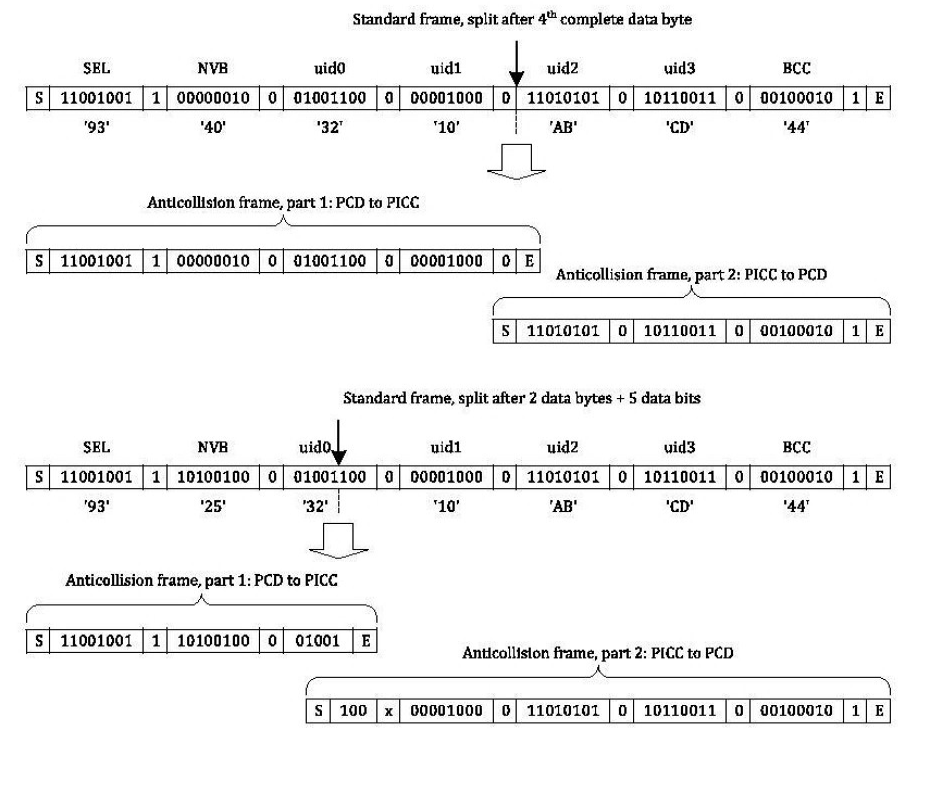
\includegraphics[scale=0.5]{./img/anticollision_frames}
  \caption{Trama Anticolisión orientada a bits~\cite[Modificaciones Mías]{iso14443-3}}
  \label{fig:anticollision}
\end{figure}

Unas de las tramas definidas en la norma terminan con un CRC16 (Cyclic Redundancy Check de 16 bits). El CRC16 permite el receptor de la trama determinar si el contenido fue corrompido. El polinomio del CRC es $P\left(x\right) = x^{16} + x^{12} + x^{5} + 1$, y el valor inicial es 0x6363~\cite{iso14443-3}\cite{iso13239}.

Cada PICC tiene un UID (Unique Identifier) que el PCD puede utilizar para enumerar todas las PICCs en su campo electromagnético y elegir cuáles activar. A pesar de que el nombre indique que el ID es único, no tiene que ser así. Está permitido usar un ID aleatorio (RID), o un ID no único (NUID). Los UIDs pueden ser: simples (4 bytes), dobles (7 bytes), o triples (10 bytes). Es requerido que todas las PICCs presentes en el campo de un PCD tienen UIDs únicos. Cuando se usan PICCs con NUIDs o RIDs es posible que haya conflictos. Debido a la gran cantidad de NUIDs posibles, la probabilidad de conflictos es mínima en un sistema bien diseñado.

Para identificar las PICCs presentes y activarlas, la norma define cinco comandos y sus respuestas, mostrados en el \tabref{tab:tramas}. La \figref{fig:14443-3-state-machine} especifica cómo una PICC debería responder cuando recibe un comando dependiendo de su estado actual.

\begin{table}[htb]
  \centering
  \begin{tabular}{l l l | l l l}
    \multicolumn{3}{c|}{\textbf{PCD $\rightarrow$ PICC}} & \multicolumn{3}{c}{\textbf{PICC $\rightarrow$ PCD}} \\
    \hline
    \textbf{Solicitud} & \textbf{Tipo} & \textbf{CRC} & \textbf{Respuesta} & \textbf{Tipo} & \textbf{CRC} \\
    \hline
    REQA & Corta & No & ATQA & Estándar & No \\
    WUPA & Corta & No & ATQA & Estándar & No \\
    ANTICOLLISION & Anticolisión & No & ANTICOLLISION & Anticolisión & No \\
    SELECT & Estándar & Sí & SAK & Estándar & Sí \\
    HLTA & Estándar & Sí & Sin Respuesta &  &  \\
  \end{tabular}
  \caption{Solicitudes y respuestas definidas en ISO/IEC 14443-3A}
  \label{tab:tramas}
\end{table}

\begin{figure}[htb]
  \centering
  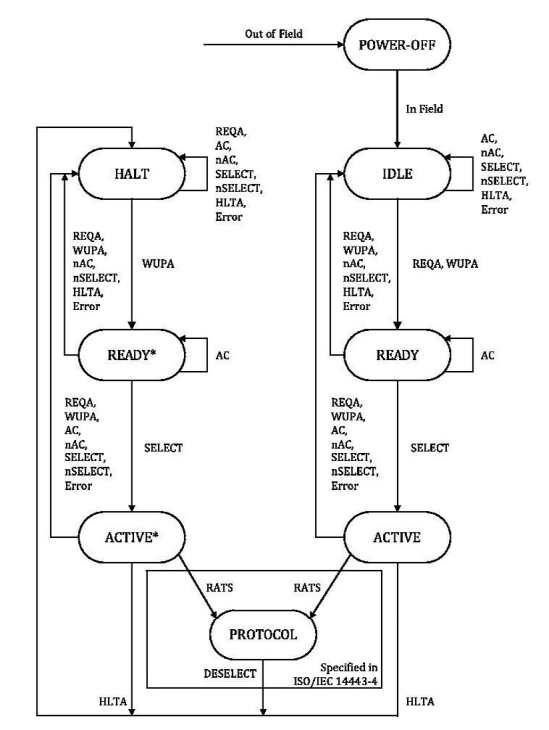
\includegraphics[scale=1]{./img/state_machine}
  \caption{Diagrama de transiciones de estados~\cite{iso14443-3}}
  \label{fig:14443-3-state-machine}
\end{figure}

\FloatBarrier

Cuando una PICC entra en un campo electromagnético, comienza en el estado IDLE. Un comando REQA o WUPA cambia el estado a READY. En ese estado el PCD puede enviar comandos de ANTICOLLISION para determinar el UID de una de las PICCs presentes. Con ese UID el PCD puede enviar un SELECT para mover la PICC al estado ACTIVE. Desde aquí el PCD puede enviar un RATS para terminar activando la PICC. En el caso de recibir un error, o un comando no esperado, la PICC vuelve al estado IDLE. Hay tres otros estados también: HALT, READY* y ACTIVE*. Las diferencias únicas entre estos estados y IDLE, READY y ACTIVE, son: WUPA es el único comando aceptado en HALT y el comando REQA es ignorado, y un error o un comando no esperado recibido en READY* o ACTIVE* causa la PICC volver a HALT en vez de IDLE. La ventaja de esto es que si el PCD decide que no quiere activar una PICC particular, puede ponerla en el estado HALT, y enviando un nuevo REQA comenzará el proceso de inicialización de nuevo en todos las PICCs menos aquellos que están en HALT.

En el caso de una PICC con UID doble el proceso de ANTICOLLISION y SELECT tiene que repetir dos veces antes de que la PICC se mueva al estado ACTIVE. En el primer lazo, los mensajes usan los primeros tres bytes de su UID junto con una etiqueta cascada: CT (Cascade Tag). La PICC responde al SELECT especificando que su UID no está completo todavía, y el lazo comienza de nuevo, esta vez usando los últimos cuatro bytes del UID. Por una PICC con UID triple este proceso tiene tres lazos. La \figref{fig:cascade_levels} muestra este proceso.

\begin{figure}[htb]
  \centering
  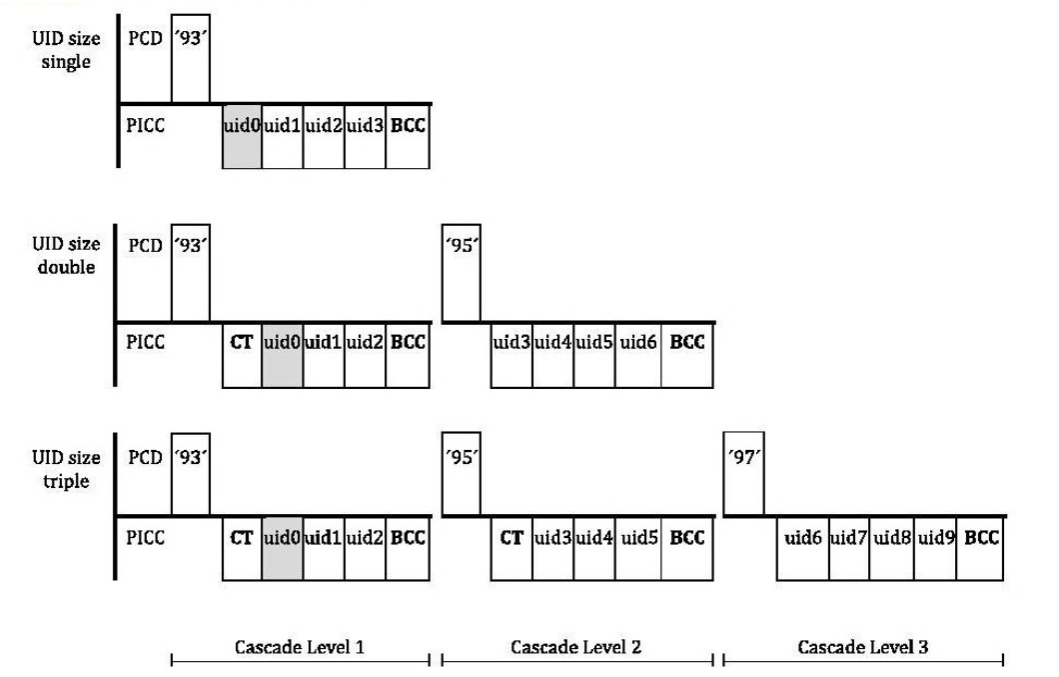
\includegraphics[scale=0.75]{./img/cascade_levels}
  \caption{Niveles cascadas para UIDs simples, dobles y triples~\cite{iso14443-3}}
  \label{fig:cascade_levels}
\end{figure}

El comando de ANTICOLLISION funciona de la siguiente forma: el PCD envía un UID parcial, y todas las PICCs en el campo electromagnético cuyas UIDs corresponden con la parte enviada, responden con los demás bits de sus UIDs. Debido al FDT fijo todas las PICCs comienzan responder de forma sincronizada. Las respuestas tienen codificación Manchester, por lo tanto cuándo dos PICCs envían valores lógicos diferentes el PCD puede detectar la colisión porque hay modulación durante todo el tiempo de bit. De esta manera el PCD sabe qué parte del UID es compartido entre todas las PICCs, y usando una búsqueda binaria puede determinar el UID completo de una de las PICC presentes. Esa PICC entonces puede ser activada o puesta en el estado HALT, y después el PCD puede repetir el proceso para enumerar todas las demás PICCs.

\FloatBarrier
\subsection{ISO/IEC 14443-4: \large{Protocolo de Transmisión}}

La mayor parte de esta subsección es común para PICCs tipo A y B, sin embargo hay dos comandos extras para terminar activando el protocolo para PICCs de tipo A. Estos comandos son RATS y PPS. El PCD debería enviar un RATS como el primer comando después de que una PICC entra en el estado ACTIVE o ACTIVE*. En el RATS el PCD asigna un CID (Card Identifier) a la PICC, esto es un identificador que el PCD puede usar para direccionar un mensaje a una PICC en particular, así que el CID debe ser único para cada PICC activa. En diferencia al UID, el CID solo tiene cuatro bits y son asignados  al momento de la inicialización y no en la  de fabricación. Este CID es válido sólo hasta que la PICC es desactivada. La respuesta al RATS es la ATS lo que contiene información sobre la capacidad de la PICC, por ejemplo las tasas de bits y el tamaño máximo de una trama que la PICC puede recibir. El comando PPS es opcional, y solo puede ser enviado inmediatamente después de que el PCD recibe la ATS. El PPS permite al PCD configurar las tasas de bits de comunicaciones en cada dirección.

La norma define dos formatos de bloques: estándares y aumentados. Bloques estándares están enviados en tramas estándares con el CRC16 presente. Bloques aumentados comienzan con el largo del bloque, y terminan con un CRC32, y el campo INF contiene códigos Hammings para la corrección de errores. La \figref{fig:std_enhanced_blocks} muestra los dos. Comunicaciones comienza con bloques estándares hasta que el PCD configura lo contrario.

\begin{figure}[htb]
  \centering
  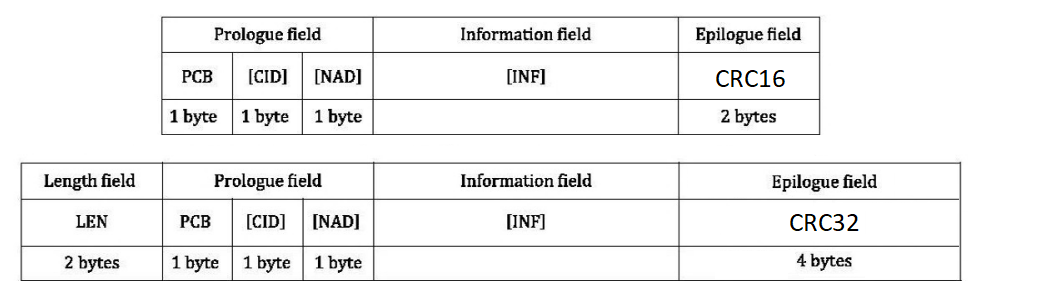
\includegraphics[scale=0.52]{./img/bloque_formats}
  \caption{El formato de un bloque estándar (arriba) y uno aumentado (abajo)~\cite{iso14443-4}}
  \label{fig:std_enhanced_blocks}
\end{figure}

Hay tres tipos de bloques: I (Information), R (Receive Ready) y S (Supervisory). El campo PCB indica que tipo de bloque es. El CID es la dirección de la PICC y solo está presente si la PICC lo soporta. El campo CID en respuestas también contiene dos bits con información sobre el nivel de potencia recibido, el PCD puede usar esa información para controlar la potencia transmitida por el campo. La NAD (Node Address) permite una PICC tener más de una aplicación, direccionado por este campo, también solo está presente si la PICC la soporta. Finalmente el campo INF contiene la información del bloque, y solo es presente por bloques tipos I y S.

Bloques-S son usados para información de control. Hay tres comandos definidos:

\begin{description}
  \item[S(WTX)] \hfill \\ Waiting Time eXtension. Si la PICC no está lista para responder a una solicitud en el tiempo permitido, puede responder con un S(WTX) pidiendo más tiempo.
  \item[S(DESELCT)] \hfill \\ Este comando es enviado por el PCD cuándo quiere desactivar la PICC.
  \item[S(PARAMETERS)] \hfill \\ Este comando está usado para leer o setear la configuración de la PICC. Por ejemplo, para cambiar la tasa de bits, o cambiar entre bloques estándares y aumentados.
\end{description}

Bloques-I son usados para transmitir información al nivel de aplicación. El protocolo de la aplicación no está definido en esta norma. Estos bloques pueden ser encadenados para permitir el envío de un mensaje más grande que el soportado por el destino, partiendo el mensaje en partes de tamaños soportados.

Bloques-R son usados para reconocer la recepción de un bloque: R(ACK) o indicar errores: R(NAK). En el caso de bloques-I encadenados un R(ACK) es enviado para pedir la siguiente parte del mensaje. También el PCD puede enviar un R(ACK/NAK) para pedir la PICC retransmita su última respuesta, esto puede ser usado para recuperar de errores. Finalmente el PCD puede enviar un R(NAK) para verificar la presencia continua de la PICC.

% ---------------------------------------------
% Descripción General del Proyecto Marco
% ---------------------------------------------

\FloatBarrier
\chapter{Descripción General del Proyecto Marco}

Este trabajo se enmarca en un proyecto que tiene como objetivo general desarrollar un circuito integrado capaz de tomar muestras de un sensor MOSFET de radiación y transmitirlas a un dispositivo externo mediante un protocolo propietario implementado encima de la norma ISO/IEC 14443A. Este proyecto marco requiere cinco bloques como se muestra en la \figref{fig:entire_project}:

\begin{figure}[htb]
  \centering
  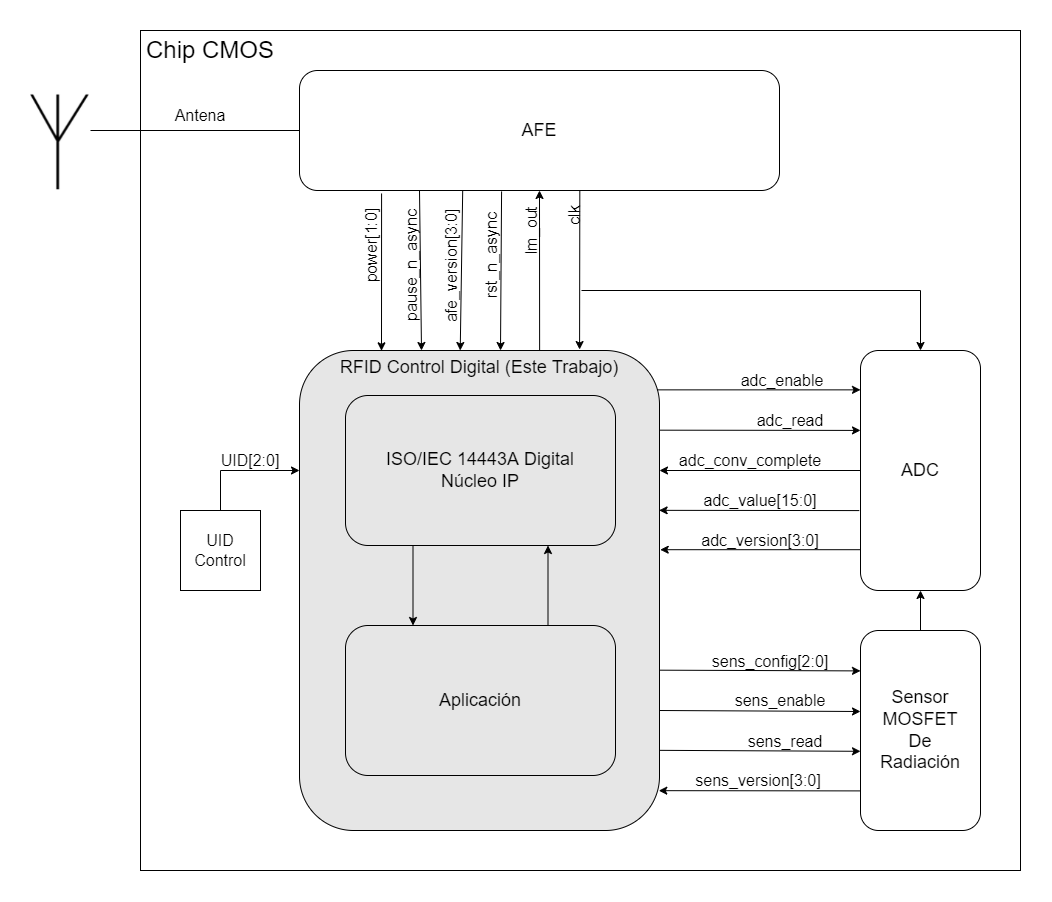
\includegraphics[width=0.95\textwidth]{./img/entire_project_v2}
  \caption{Diagrama general del proyecto marco y su relación con el bloque a diseñar en esta Tesis.}
  \label{fig:entire_project}
\end{figure}

\begin{description}
  \item[El Analogue Front End (AFE)] \hfill \\ Es la parte analógica de la norma ISO/IEC 14443A-2.
  \item[El sensor MOSFET de radiación] \hfill \\ Desarrollado por el Laboratorio de Física de Dispositivos-Microelectrónica (LFDM) de la facultad de ingeniería de la UBA.
  \item[El Conversor Analógico Digital (ADC, por sus siglas en inglés)] \hfill \\ Encargado de convertir la salida analógica del sensor a una señal digital.
  \item[El RFID Control Digital] \hfill \\ Es el objetivo de esta Tesis.
  \item[El UID Control] \hfill \\ Permite asignar la parte variable del UID de la PICC.
\end{description}

Algunos de estos bloques no se han desarrollado todavía, por lo que es necesario asumir las especificaciones de los mismos.

El AFE es responsable de:

\begin{itemize}
  \item Recibir y regular potencia desde el campo electromagnético. La implementación de esta tesis se realiza considerando la tecnología de fabricación de XFAB 180 nm, la cual utiliza celdas estándares que requieren una tensión de 1.8 V, por lo que el AFE debe producir esa tensión, y mantenerla durante las pausas.
  \item Recuperar la señal de reloj a partir de la portadora. La dificultad en este punto reside en el hecho de que el PCD envía información a la PICC utilizando pausas en la portadora, por lo cual se espera que el reloj se detenga durante estas pausas. Es posible utilizar un PLL para producir un reloj continuo. El circuito de esta tesis es elaborado con habilidad para funcionar con un reloj continuo o con un reloj que se detenga durante las pausas. En la \secref{sec:sequence_decode}{sequence\_decode} se detalla el número máximo de flancos del reloj que es posible perder conservando una correcta decodificación de las secuencias.
  \item Manejar la señal de reset (activa baja). Los demás bloques se deben mantener en un estado de reset hasta que la tensión de alimentación sea estable.
  \item Detectar las pausas enviadas desde el PCD.
  \item Permitir la transmisión de respuestas al PCD mediante un modulador de carga. El modulador debería ser manejado directamente desde una entrada del bloque, lo cual sería conectado a la salida \textit{lm\_out} del bloque RFID Digital Control. La señal se obtiene como el AND lógico de la codificación Manchester y la subportadora.
  \item Generar una señal indicando el nivel de potencia recibida a través del campo electromagnético (opcional). Si se tiene esta información, la misma puede ser enviada al PCD en el campo CID de mensajes de nivel protocolo. El PCD puede usarla para ajustar la intensidad del campo electromagnético.
  \item Proveer una salida de cuatro bits que indique la versión del hardware del AFE. Este valor forma parte de la información enviada al PCD como respuesta al mensaje de protocolo IDENTIFY.
\end{itemize}

El sensor de radiación tiene tres entradas: \textit{sens\_config[2:0]}, \textit{sens\_enable} y \textit{sens\_read} . Para leer el sensor, primero se debe establecer el valor de \textit{sens\_config[2:0]} de manera que se elija la configuración del sensor deseado por el usuario. Posteriormente se debe establecer \textit{sens\_enable} en ‘1’ para activar el sensor. Finalmente después del tiempo deseado por el usuario, llevar \textit{sens\_read} a ‘1’ configura al circuito del sensor en modo lectura para su muestreo. Por otro lado, el sensor tiene dos salidas, una analógica que está conectada al ADC, y una señal de cuatro bits que indica la versión del sensor. Este valor forma parte de la información enviada al PCD como respuesta al mensaje de protocolo IDENTIFY.

Por su parte el ADC, además de la entrada analógica proveniente desde el sensor, tiene otras dos entradas: \textit{adc\_enable} y \textit{adc\_read}. El flanco ascendente de la señal \textit{adc\_read} indica el momento de muestreo de la salida del sensor.. Respecto de las salidas, hay tres: \textit{adc\_conversion\_complete}, \textit{adc\_value[15:0]} y \textit{adc\_versión[3:0]}. Cuando el ADC completa la conversión la señal \textit{adc\_conversion\_complete} toma el valor '1' durante un ciclo del reloj. La señal \textit{adc\_value} debe ser estable antes del pulso en \textit{adc\_conversion\_complete}.

El bloque de UID Control es responsable de especificar los tres bits más bajos del UID de la PICC. Este valor puede ser configurado mediante una memoria no volátil, pero en esta tesis la intención es configurarlo utilizando wire bonding o resistores pull up/down.

El objetivo de esta tesis es implementar el bloque del RFID Control Digital, que consiste en dos sub-bloques: Una implementación del parte digital de la norma ISO/IEC 14443A y un protocolo a nivel aplicación que permita la lectura del sensor y envíe esta información al PCD. Un requisito de este bloque es que la entrada de UID se mantenga estable mientras el bloque no esté en un estado de reset.

% --------------------------------------------
% Implementación y Verificación
% ---------------------------------------------

\FloatBarrier
\chapter{Implementación y Verificación}

La implementación de todos los módulos y los bancos de prueba se escriben con el HDL (Hardware Description Language) SystemVerilog, el cual  es definido en IEEE 1800~\cite{ieee1800}. SystemVerilog es basado en Verilog,  formalmente definido en IEEE 1364~\cite{ieee1364}. SystemVerilog es conocido principalmente como un HDL para verificación debido a sus extensiones sustanciales a verilog en ese ámbito, por ejemplo en la adicción de conceptos de programación orientados a objetivos (como clases), y aserciones. Además SystemVerilog tiene varias ventajas a Verilog para uso en síntesis~\cite{synthesisable_sv}, por ejemplo:

\begin{description}
  \item[Enumeraciones (enum) y estructuras (struct)] \hfill \\ Como en el lenguaje de programación C.
  \item[always\_comb y always\_ff] \hfill \\ Estos permiten al ingeniero especificar su intención a implementar lógica combinatoria o secuencial respectivamente. Las herramientas pueden verificar que el circuito inferido cumple con esa intención, por ejemplo, que los bloques combinatorios no contienen latches.
  \item[Interfaces] \hfill \\ Colecciones de señales que son frecuentemente usadas juntas para reducir la replicación de código.
\end{description}

La implementación de esta tesis está dividida en dos: 1) El núcleo IP genérico para ISO/IEC 14443A que es la lógica digital necesaria para recibir, decodificar y actuar sobre los mensajes definidos en la norma, y construir, codificar y transmitir las respuestas adecuadas. Este núcleo IP está dividido en tres partes principales, uno para cada parte de la norma (excepto ISO/IEC 14443-1). 2) El sistema de control del sensor y del ADC. La \figref{fig:top_level} muestra todos esos bloques, y el flujo de datos entre ellos.

\begin{figure}[htb]
  \centering
  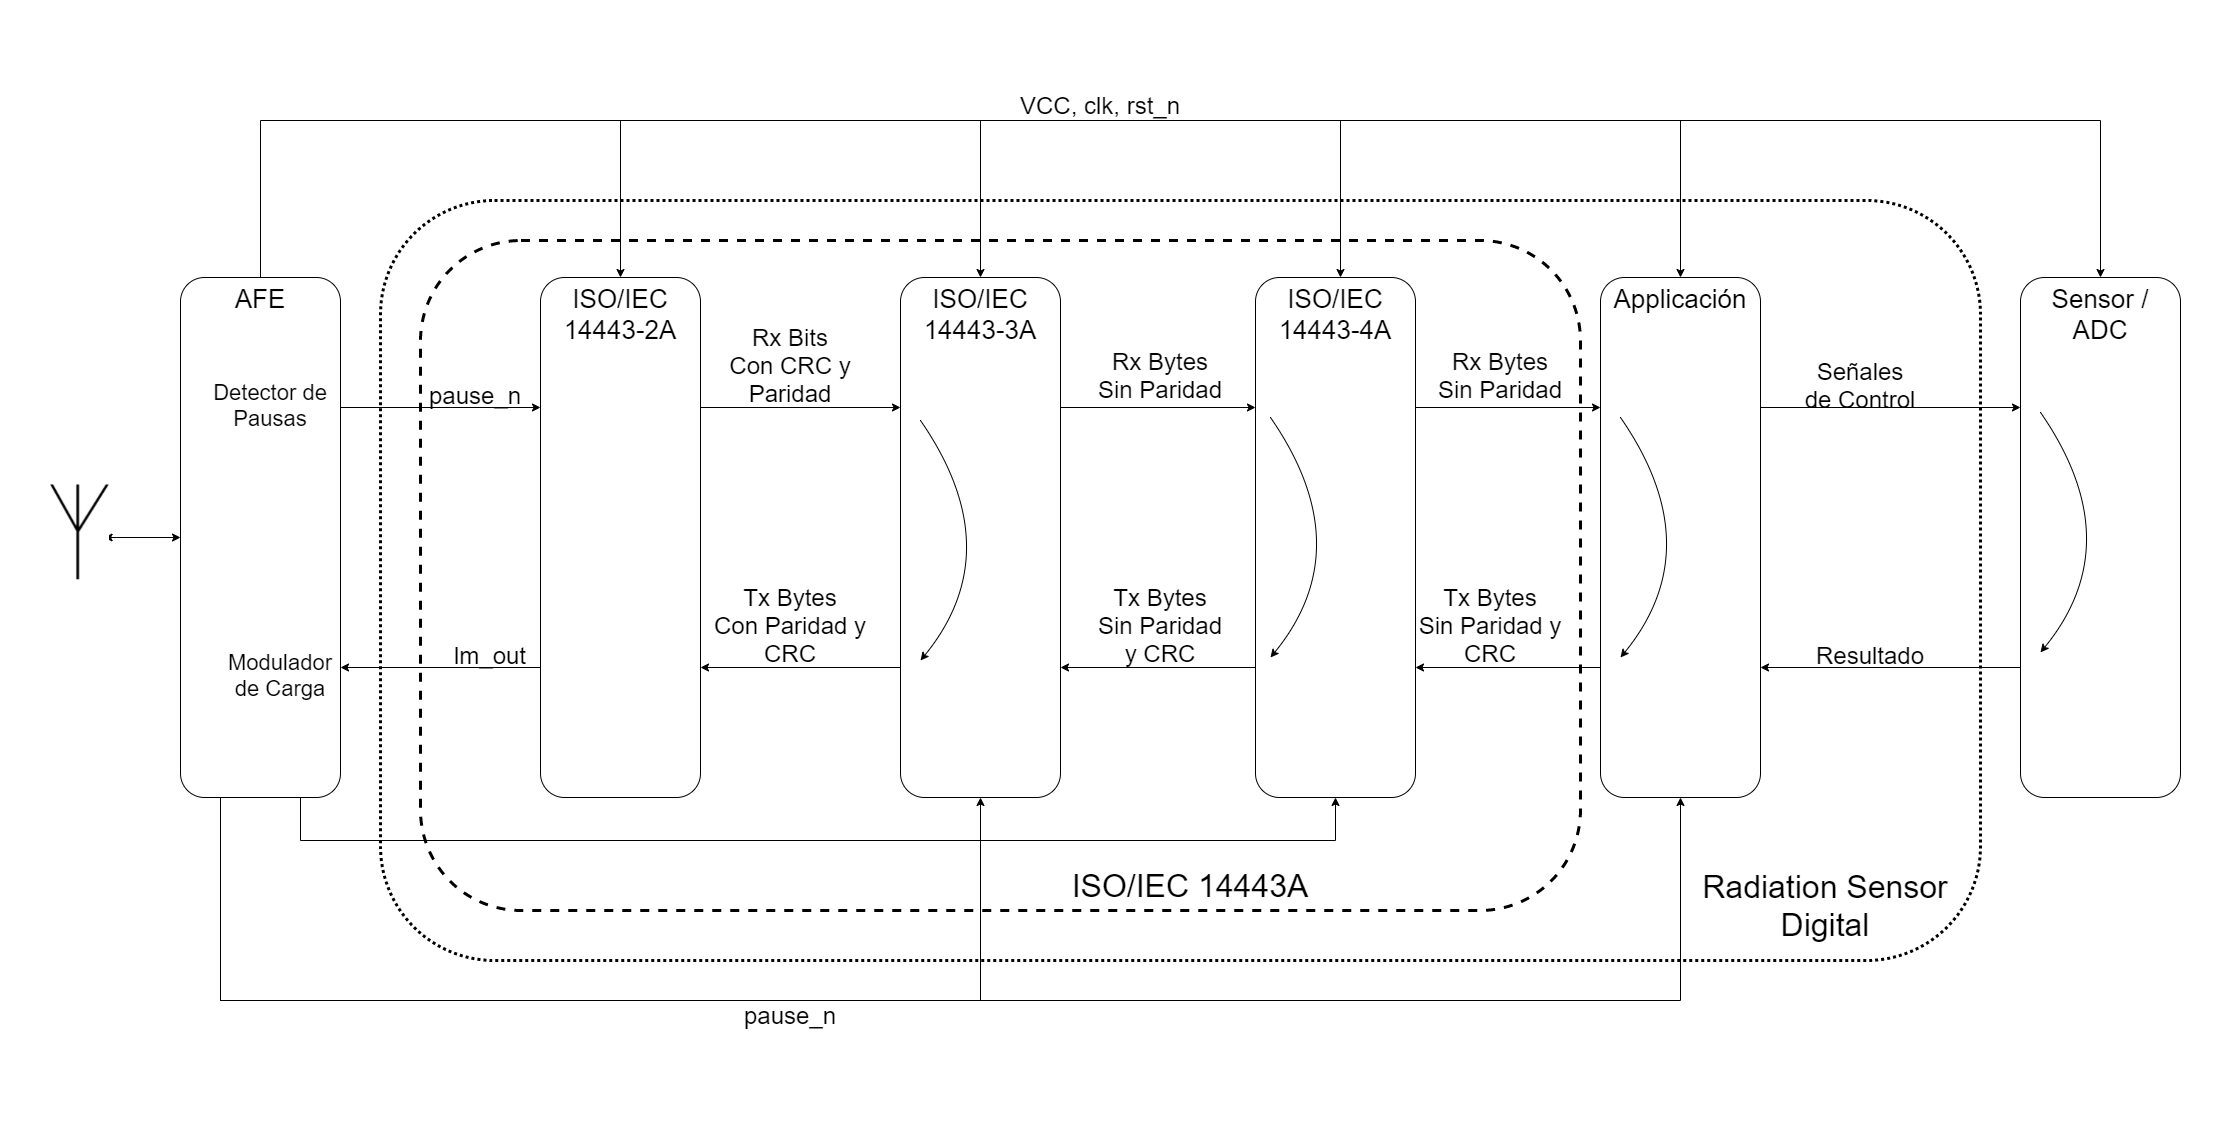
\includegraphics[width=1.0\textwidth]{./img/top_level}
  \caption{Los bloques principales de la implementación.}
  \label{fig:top_level}
\end{figure}

% Interfaces
% --------------------------------
\FloatBarrier
\section{Interfaces}

La norma IEEE de SystemVerilog define un interfaz como:

\begin{displaycquote}[traducción mía]{ieee1800}
A su nivel más bajo, un interfaz es un conjunto nombrado de nets o variables. La interfaz es instanciada en un diseño y puede ser accedida por un puerto como un ítem sencillo; las nets o variables componentes [pueden ser] referidos cuando sea necesario. Una proporción significativa de un diseño verilog frecuentemente consiste en listas de puertos y listas de conexiones, los que son simplemente repeticiones de nombres. La habilidad de reemplazar un grupo de nombres con un nombre simple puede reducir significativamente el tamaño de una descripción y mejorar su mantenibilidad. 
\end{displaycquote}

Además de esas ventajas, una interfaz puede contener funcionalidad, sea para síntesis o verificación, por ejemplo se puede agregar aserciones que verifican el comportamiento de los nets internos en vez de tener que duplicar esas pruebas en cada sitio que la interfaz es usada. Una interfaz puede tener una o más modports, los que especifican las direcciones de las señales. Esos modports pueden ser usados en la lista de puertas por un módulo en vez de especificar cada señal y su dirección individualmente.

Este trabajo consiste en varios módulos que contienen uno o más sumideros para recibir tramas desde otros módulos, y una o más fuentes para enviar tramas a otros módulos. Por ejemplo el módulo: \textbf{frame\_decode} recibe tramas desde el módulo: \textbf{sequence\_decode}, quita los bits de paridad, y reenvía las tramas modificadas al módulo: \textbf{deserialiser}. Por lo tanto muchos de los módulos manejan el mismo conjunto de señales, lo que es el uso principal por interfaces. Hay dos interfaces definidas en este trabajo, uno para la recepción de tramas (\textit{rx\_interface}), y otra para la transmisión de las respuestas (\textit{tx\_interface}). Las dos son parametrizadas para funcionar con series de bits o de bytes. Las interfaces son usadas para conectar una fuente en un módulo a un sumidero en otro módulo.

La \textit{rx\_interface} contiene:

\begin{itemize}
  \item \textit{soc}: Un indicador que indica el comienzo de una trama.
  \item \textit{eoc}: Un indicador que indica el fin de una trama.
  \item \textit{data}: Un bit / byte de la trama.
  \item \textit{data\_valid}: Un indicador que indica si los datos en \textit{data} son válidos.
  \item \textit{data\_bits}: La cantidad de bits válidos. Por una interfaz configurada a bytes, esta señal permite la recepción de tramas cortas que tienen solo 7 bits, o de tramas anticolisión orientada a bits que pueden terminar con entre uno y ocho bits.
  \item \textit{error}: Indica la detección de un error en la trama, por ejemplo: un bit de paridad equivocado.
\end{itemize}


La \figref{fig:rx_iface} muestra una simulación de la recepción de una trama corta con una \textit{rx\_interface} de bits, y su conversión a una serie de bytes. Arriba están las señales en una \textit{rx\_interface} de bits, \textit{data\_valid} está en ‘1’ siete veces durante la trama, indicando que el dato recibido es: 1,1,1,1,0,1,0. Debido a que el bit menos significativo es enviado primero, este serie representa 7’b0101111. Abajo están las señales en una \textit{rx\_interface} de bytes representando la misma trama. El dato tiene valor 8’bX0101111 cuando \textit{data\_valid} tiene valor lógico igual a ‘1’.

La \textit{rx\_interface} incluye varias aserciones para verificar el comportamiento de las señales en la interfaz. Las aserciones consideran: Las señales son correctas en el estado de reset, los indicadores nunca son desconocidos, \textit{soc} y \textit{eoc} no están en ‘1’ en el mismo ciclo, y que solo están en ‘1’ por la duración de un solo ciclo del reloj a la vez.

\begin{figure}[htb]
  \centering
  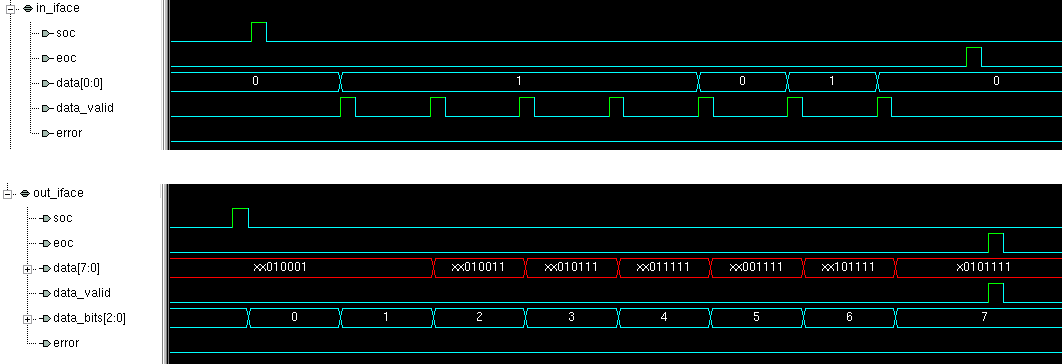
\includegraphics[width=1.0\textwidth]{./img/rx_iface_example}
  \caption{Una simulación de la recepción de una trama corta representada con una \textit{rx\_interface} de bits (arriba) y su conversión a una \textit{rx\_interface} de bytes (abajo).}
  \label{fig:rx_iface}
\end{figure}

\FloatBarrier

La \textit{tx\_interface} contiene:

\begin{itemize}
  \item \textit{data}: Un bit / byte de la trama.
  \item \textit{data\_valid}: Un indicador que indica que \textit{data} es válida.
  \item \textit{data\_bits}: La cantidad de bits válidos. Para una interfaz configurada a bytes, esta señal permite la transmisión de tramas de anticolisión orientada a bits, las que pueden comenzar con un byte parcial.
  \item \textit{last\_bit\_in\_byte}: Esta señal solo existe en interfaces de bits. Indica que el bit actual es el último bit en un byte. Es usada para conocer dónde agregar bits de paridad dentro de una serie de bits.
  \item \textit{req}: El sumidero usa esta señal para pedir que la fuente envíe el siguiente bit / byte de la trama. La norma ISO/IEC 14443A-2 define la duración de bits como 128 ciclos de la portadora, por lo tanto esta señal es necesaria para limitar la tasa de envío de datos.
\end{itemize}

Cuándo una fuente está lista para transmitir una trama se establece el primer bit / byte de la trama en la señal \textit{data} y fija \textit{data\_valid} en ‘1’. El sumidero puede utilizar la señal \textit{data\_valid} para ver si la fuente tiene data enviar. Después de haber leído la primera bit / byte de data, el sumidero fija la señal \textit{req} en ‘1’ durante un ciclo del reloj. La fuente detecta ese pulso y si hay más data a enviar, se actualiza la \textit{data} con el siguiente bit / byte, dejando \textit{data\_valid} en ‘1’. Este proceso repite hasta que la fuente no tiene más data a enviar, y después del último pulso en la \textit{req}, se fija \textit{data\_valid} en ‘0’. La \figref{fig:tx_iface} muestra una simulación de la transmisión de una trama de 16 bits con una \textit{tx\_interface} de bytes, y su conversión a una serie de bits. Arriba están las señales en la \textit{tx\_interface} de bytes enviando la data 0xAE, 0x42. Abajo están las señales en una \textit{tx\_interface} de bits representando la misma trama.

La \textit{tx\_interface} también incluye tres aserciones que verifican: Las señales son correctas en el estado de reset, \textit{req} es ‘1’ solo para la duración de un ciclo del reloj, y que \textit{data}, \textit{data\_valid}, \textit{data\_bits} y \textit{last\_bit\_in\_byte} solo cambian estado cuando \textit{data\_valid} está ‘0’ o en los cuatro ciclos después de un pulso de req. La última aserción es para verificar que la fuente puede proveer datos cuándo es pedido con la señal \textit{req} antes de que el sumidero la necesita.

\begin{figure}[htb]
  \centering
  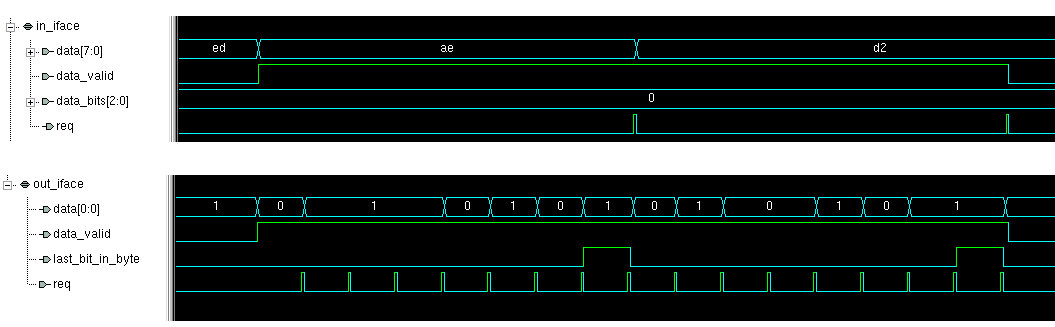
\includegraphics[width=1.0\textwidth]{./img/tx_iface_example}
  \caption{Una simulación de la transmisión de una trama de 16 bits representada con una \textit{tx\_interface} de bytes (arriba) y su conversión a una \textit{tx\_interface} de bits (abajo).}
  \label{fig:tx_iface}
\end{figure}


% Marco de Verificación
% --------------------------------
\FloatBarrier
\section{Marco de Verificación}

Simulación y verificación es una parte muy importante del diseño digital. En un informe de 2020 sobre las tendencias de diseño y verificación de ICs y ASICs~\cite{verification_trends_2020}, los autores encontraron que en promedio más de 50\% del tiempo de un proyecto es utilizado en verificación. También encontraron que en promedio hay un ingeniero de verificación por cada ingeniero de diseño, además los ingenieros de diseño gastan aproximadamente la mitad de su tiempo verificando sus diseños.

En esta tesis se utiliza verificación funcional mediante simulaciones con la herramienta VCS de Synopsys. Las simulaciones son completamente automatizadas y son ejecutadas con un comando sencillo utilizando un Makefile, por ejemplo: “make serialiser\_tb”.

UVM (Universal Verification Methodology) es una metodología de verificación funcional mediante un conjunto de clases de SystemVerilog. Aproximadamente 75\% de proyectos mundiales son verificados con UVM~\cite{verification_trends_2020}. Una de las ventajas principales de UVM es la modularidad. El código es partido en bloques separados facilitando la reutilización de los componentes en varios bancos de pruebas sin tener que duplicar código. La desventaja principal es la complejidad, requiere mucho código para armar un banco de prueba. UVM no es usada en esta tesis porque su implementación sería más compleja que el propio diseño. Sin embargo el marco de verificación está basado en las técnicas de UVM.

El proceso de verificación es estimular las entradas del DUT (Design Under Test) y verificar que las salidas son las esperadas. Frecuentemente no es posible verificar un diseño para todas las combinaciones y secuencias posibles de las entradas, por lo tanto es común usar estímulo aleatorio. Con estímulo aleatorio siempre hay el riesgo de no verificar parte del diseño, por la posibilidad de no elegir una de las combinaciones o secuencias de entradas necesarias para estimular esa parte del diseño. Una técnica para ayudar a mitigar esto, es: aleatorio restringido (constrained random), esta técnica permite la generación de estímulo aleatorio mediante constraints para restringir el estímulo a un rango interesante en particular. Por ejemplo, en vez de generar tramas completamente aleatorias, pueden ser limitadas: a tramas válidas, una colección de tramas en particular, o tramas con errores.

Una técnica para asegurar que todas las partes de un diseño son verificadas suficientemente, es generar informes de cobertura. La herramienta VCS está habilitada para generar, de forma automática, informes de cobertura de código con varias métricas, y un resultado total de qué proporción del diseño fue verificado. Estos informes pueden ser analizados por el diseñador para verificar cuáles partes de su diseño fue suficientemente estimulado y cuáles partes necesitan más trabajo. Las métricas de cobertura de código habilitadas en VCS son:

\begin{itemize}
  \item Línea: Muestra las líneas del RTL que fueron ejecutadas.
  \item Condición: Muestra las sub expresiones booleanas que fueron evaluados a verdadero y falso. Por ejemplo en la declaración: “res = (A == 0) ? B : C”, el informe de cobertura indicará si la expresión “A == 0” fue evaluado al menos una vez a verdadero y al menos una vez a falso.
  \item Cambio de Estado (Toggle): Muestra cuáles señales y puertas cambiaron de estado en las dos direcciones.
  \item Branch: Muestra cuáles branches fueron tomados.
  \item FSM (Finite State Machine): Muestra cuáles estados en un FSM fueron utilizados, y las transiciones entre ellos.
  \item Aserción: Muestra cuáles aserciones fueron: ejecutadas, aprobadas y falladas, y cuántas veces por cada uno.
\end{itemize}

El marco de verificación es implementado con varios componentes, la mayoría son clases de SystemVerilog. Los componentes pueden ser divididos en siete grupos distintos:

\begin{itemize}
  \item Transacciones: Una transacción representa una trama, puede ser una trama de bits, de bytes o de secuencias (como definido en ISO/IEC 14443-2).
  \item Controladores: Un controlador envía una transacción sobre una interfaz.
  \item Monitores: Un monitor monitoriza una interfaz, y construye transacciones representando las tramas detectadas.
  \item Generador de transacciones: Genera transacciones de bytes para representar las tramas definidas en la norma. También puede generar transacciones aleatoriamente.
  \item Convertidor de transacciones: Produce una transacción en un formato desde una transacción en otro formato. Por ejemplo puede convertir una transacción de bytes a una transacción de bits, opcionalmente agregando los bits de paridad.
  \item Secuencias: Código compartido para verificar diseños que reciben tramas, actúan sobre ellos, y generan las respuestas. Por ejemplo: cuándo el DUT está en el estado READY, responde a un SELECT con un SAK con los valores esperados, y se transiciona al estado ACTIVE. Ese ejemplo es una prueba utilizada para verificar el comportamiento de cuatro módulos: \textbf{initialization}, \textbf{iso14443\_3a}, \textbf{iso14443a}, \textbf{radiation\_sensor\_digital\_top}.
  \item Otros: Este grupo incluye: modelos de los bloques analógicos, una clase para guardar la dirección de una PICC (UID, CID y NAD), y unas interfaces que solo están usadas para verificación.
\end{itemize}

% Transacciones
\FloatBarrier
\subsection{Transacciones}

La \figref{fig:transaction_uml} muestra un diagrama UML (Unified Modelling Language) de las clases de transacciones. La clase base es \textbf{Transaction}, es abstracta y contiene dos métodos abstractos: \textbf{compare()} que evalúa si dos transacciones son iguales, y \textbf{to\_string()} que devuelve un string describiendo la transacción. La clase \textbf{QueueTransaction} extiende \textbf{Transaction}, tiene un parámetro de tipo: \textit{ElemType}, que especifica el tipo de una cola declarada en la clase. La cola es usada para contener el dato de la trama representada por la transacción. Los dos métodos abstractos de \textbf{Transaction} son sustituidos, y hay métodos extras para ayudar con la construcción de transacciones. Hay tres clases que extienden \textbf{QueueTransaction}: \textbf{ByteQueueTransaction}, \textbf{BitQueueTransaction} y \textbf{PCDPauseNTransaction}, que definen el parámetro \textit{ElemType} como: logic[7:0] (byte), logic (bit) y \textbf{PCDBitSequence} respectivamente. \textbf{PCDBitSequence} es una enum definida en un paquete, y consiste en las secuencias X, Y y Z describidas en la sección ? (14443-2A). \textbf{ByteQueueTransaction} tiene métodos para calcular y agregar CRCs a la transacción, y para convertir la transacción a una cola de bits. \textbf{BitQueueTransaction} tiene un método para agregar los bits de paridad.

\begin{figure}[htb]
  \centering
  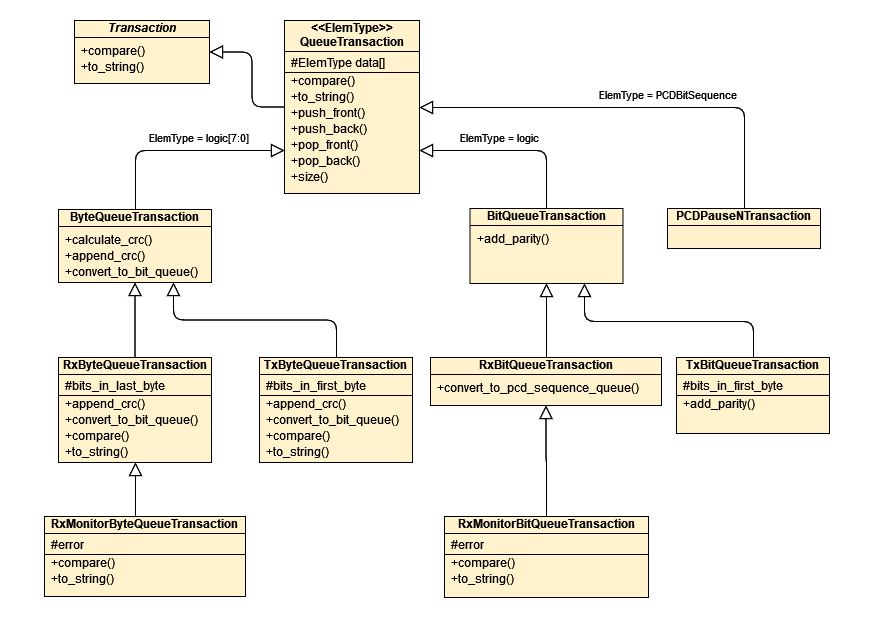
\includegraphics[width=1.0\textwidth]{./img/transactions_uml.vpd}
  \caption{Diagrama UML de clases de transacciones.}
  \label{fig:transaction_uml}
\end{figure}

Para transacciones de transmisión (PICC a PCD), hay dos clases \textbf{TxByteQueueTransaction} y \textbf{TxBitQueueTransaction}, las dos tienen un atributo especificando cuántos bits hay en el primer byte, eso es porque respuestas a mensajes de ANTICOLISIÓN pueden comenzar con un byte parcial, como se muestra en la \figref{fig:anticollision}.

Para transacciones de recepción (PCD a PICC), hay cuatro clases en adición a \textbf{PCDPauseNTransaction}: \textbf{RxByteQueueTransaction}, que tiene un atributo especificando cuántos bits hay en el último byte para tramas cortas y de anticolisiones que pueden terminar con un byte parcial. \textbf{RxBitQueueTransaction}, que tiene un método para convertir su data a una cola de \textbf{PCDBitSecuences}. Estas dos clases son usadas en los controladores para enviar transacciones a los DUTs. Las otras dos clases son \textbf{RxMonitorByteQueueTransaction} y \textbf{RxMonitorBitQueueTransaction}, las que son son las transacciones construidos por los Monitores de recepción. Los dos tienen un atributo para indicar si el monitor ha detectado un pulso en la señal \textit{error} de las interfaces de recepción.

% Controladores
\FloatBarrier
\subsection{Controladores}

La \figref{fig:driver_uml} muestra un diagrama UML de clases para los controladores. La clase base principal es \textbf{Driver}, es abstracta y tiene dos tipos parametrizados: \textit{IfaceType}, que es el tipo de la interfaz que maneja, y \textit{TransType}, que es el tipo de las transacciones que el controlador puede envíar sobre esa interfaz. El método \textbf{start()} lleva una referencia a una cola de elementos de tipo \textbf{TransType} y comienza un nuevo hilo de ejecución. Ese hilo monitoriza la cola, cuándo una transacción es empujada a la cola desde el banco de prueba, la controladora la quita, y la pasa al método \textbf{process()}. En esta clase base \textbf{process()} es abstracto, las clases hijas lo sustituyen para definir cómo envíar la transacción sobre su interfaz.

\textbf{RxIfaceDriver} es la clase base para los controladores de las interfaces de recepción (PCD a PICC). \textbf{RxByteIfaceDriver} y \textbf{RxBitIfaceDriver} la extienden para uso con las interfaces de bytes y de bits respectivamente. Las implementaciones del método \textbf{process()} envían el SOC, los datos y el EOC. Esas clases tienen atributos para controlar el timing de las transmisiones, por ejemplo el tiempo entre el SOC y el primer dato, y entre los datos mismos. También esas clases pueden introducir errores en la transmisión pulsando la señal \textit{error} de la \textit{rx\_interface} en un sitio aleatorio.

El controlador \textbf{PCDPauseNDriver} es parecido al \textbf{RxIfaceDriver}, pero en vez de envíar transacciones sobre una \textit{rx\_interface}, las envía mediante una señal \textit{pause\_n} como haría el detector de pausas en el AFE real.

\begin{figure}[htb]
  \centering
  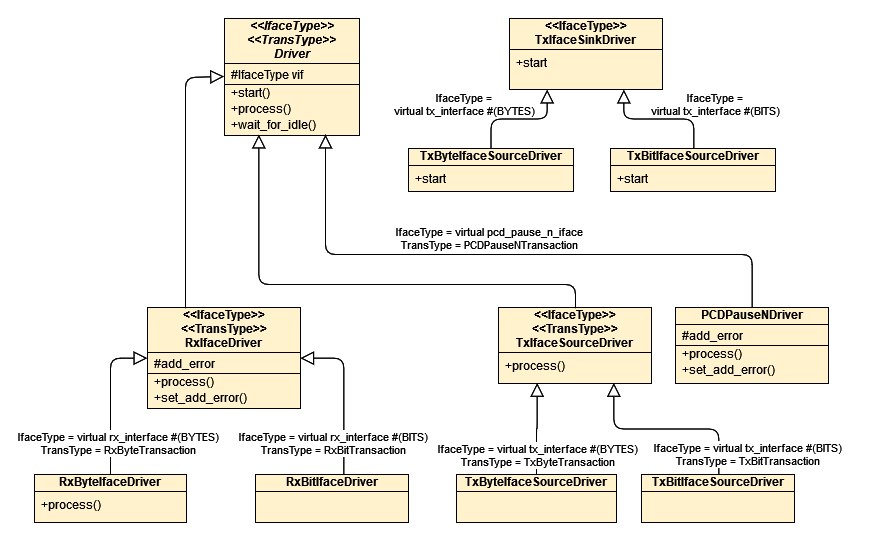
\includegraphics[width=1.0\textwidth]{./img/drivers_uml.vpd}
  \caption{Diagrama UML de clases para los controladores.}
  \label{fig:driver_uml}
\end{figure}

Los controladores de transmisión (PICC a PCD) están divididos en dos partes: las fuentes y los sumideros. Los sumideros son necesarios porque la señal \textit{req} de la \textit{tx\_interface} es manejada por el sumidero. La clase \textbf{TxIfaceSinkDriver} es la clase base de los sumideros, contiene un método \textbf{start()} que espera por la activación de la señal \textit{data\_valid} de la interfaz, y después comienza a pulsar \textit{req} periódicamente hasta que \textit{data\_valid} baja a ‘0’. Unos atributos controlan los timings de los pulsos. Las clases hijas \textbf{TxByteIfaceSinkDriver} y \textbf{TxBitIfaceSinkDriver} son usadas con una \textit{tx\_interface} de bytes y de bits respectivamente. La clase \textbf{TxIfaceSourceDriver} y sus clases hijas son los controladores de las fuentes, y funcionan de la misma manera de los controladores de recepción.

% Monitores
\FloatBarrier
\subsection{Monitores}

La \figref{fig:monitor_uml} muestra el diagrama UML de las clases para los monitores. La clase base es \textbf{Monitor}, es abstracta y tiene dos tipos parametrizados: \textit{IfaceType}, que es el tipo de la interfaz que monitoriza, y \textit{TransType}, que es el tipo de las transacciones que construye. El método \textbf{start()} lleva una referencia a una cola de elementos de tipo \textit{TransType} y comienza un nuevo hilo de ejecución. Ese hilo llama el método \textbf{process()}, si esa tarea devuelve una transacción válida, es empujada a la cola, para que el banco de prueba pueda verificarla, y el método \textbf{process()} es llamado de nuevo. Ese proceso se repite por siempre. En esta clase base \textbf{process()} es abstracto, las clases hijas lo sustituyen para definir cómo armar una transacción desde las señales de la interfaz.

\begin{figure}[htb]
  \centering
  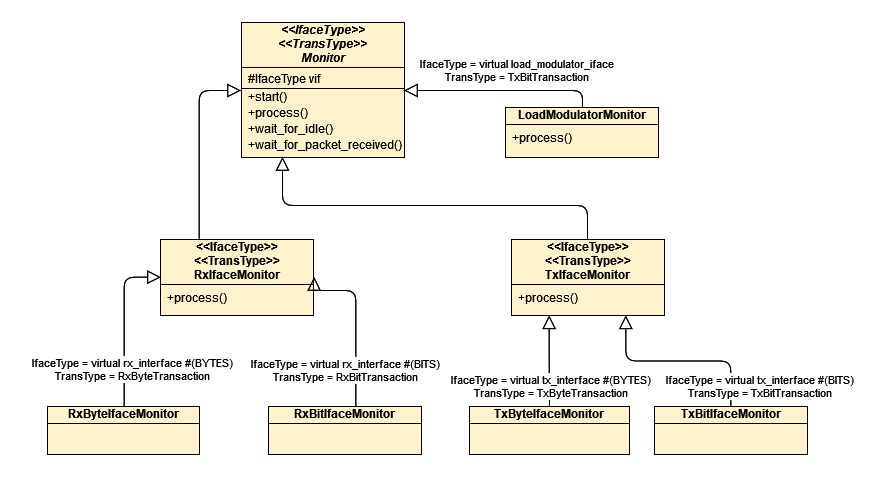
\includegraphics[width=1.0\textwidth]{./img/monitors_uml.vpd}
  \caption{Diagrama UML de clases para los monitores.}
  \label{fig:monitor_uml}
\end{figure}

Para la \textit{rx\_interface}, las clases son \textbf{RxIfaceMonitor} y sus hijas \textbf{RxByteIfaceMonitor} y \textbf{RxBitIfaceMonitor}. El método \textbf{process()} monitoriza la \textit{rx\_interface} para una de las señales: \textit{SOC}, \textit{EOC}, \textit{error} o \textit{data\_valid} tener valor ‘1’. Cuándo \textit{SOC} está en ‘1’ comienza construir una nueva transacción. Cuándo \textit{data\_valid} está en ‘1’ el bit o byte actual en la señal \textit{data} es empujado a la cola de datos en la transacción. Cuándo \textit{error} está en ‘1’ la transacción es actualizada para indicar la detección del error. Finalmente cuándo \textit{EOC} está en ‘1’ indicando el fin de la trama, la transacción es devuelta. Si detecta un error, por ejemplo un SOC dentro de una trama, o un EOC fuera de una trama, un error es indicado al usuario mediante la función de sistema \textbf{\$error()}, la transacción es abandonada, y un error es devuelto.

Los monitores para la \textit{tx\_interface} son parecidos a los monitores de recepción, salvo por el método \textit{process()}. Este método primero espera hasta que la señal \textit{data\_valid} esté en ‘1’, que indica el comienzo de una trama. Cuándo la señal \textit{req} está en ‘1’, significa que el sumidero ha leído el último dato, así el monitor agrega el bit o byte actual en la señal \textit{data} a la transacción. Cuándo \textit{data\_valid} baja a ‘0’, significa que la fuente no tiene más datos a enviar siendo el fin de la trama, y la transacción es devuelta.

Finalmente la clase \textbf{LoadModulatorMonitor} es diseñada para monitorear y decodificar la señal \textit{lm\_out} que es conectada al modulador de carga en el AFE. El método \textbf{process()} primero espera por un flanco ascendente de la señal \textit{lm\_out}, y después toma una muestra de la señal cada ciclo para 128 ciclos, lo que es la duración para enviar un bit. Si las muestras son iguales al patrón definido en la norma para envíar un ‘1’ o ‘0’ lógico, ese valor lógico es agregado a la transacción. Cuándo todas las muestras están ‘0’s indica el fin de la trama y la transacción es devuelta. Las muestras teniendo cualquier otro patrón indican un error, y el monitor llama la función de sistema \textbf{\$error()} para avisar al usuario.

% Generador y Conversores de Transacciones
\FloatBarrier
\subsection{Generador y Conversores de Transacciones}

El generador de transacciones es una clase \textbf{TransactionGenerator}, que tiene métodos para generar transacciones para todos las tramas definidas en la norma. Por tramas de recepción (PCD a PICC) las transacciones generadas son de tipo \textbf{RxByteTransactions}. Transacciones de tipo \textbf{TxByteTransactions} son generadas por tramas de transmisión (PICC a PCD). También hay métodos para generar transacciones desde una cola de bytes, y para generar transacciones aleatorias restringidas a no ser las tramas definidas en la norma. Las transacciones pueden tener CRCs agregadas automáticamente si es deseado por el usuario. Además es posible pedir que el CRC agregado sea corrompido para verificar como un módulo maneja tramas con errores de CRC.

Los conversores de transacciones son clases que facilitan la conversión de un tipo de transacción a otro. Un ejemplo del uso de un conversor de transacciones es: convirtiendo una \textbf{RxByteTransaction} generada por el generador de transacciones a una \textbf{RxBitTransaction} que el controlador \textbf{RxBitIfaceDriver} puede enviar sobre una \textit{rx\_interface} de bits. La clase base abstracta es \textbf{TransactionConverter}. Esta clase tiene dos tipos parametrizados: \textit{InputTransType} y \textit{OutputTransType} que especifican los tipos de las transacciones involucradas en la conversión. Las clases son:

\begin{itemize}
  \item \textbf{RxByteToByteTransactionConverter}: Convertir una \textbf{RxByteTransaction} a una \textbf{RxByteTransaction} (identidad).
  \item \textbf{RxByteToBitTransactionConverter}: Convertir una \textbf{RxByteTransaction} a una \textbf{RxBitTransaction}, opcionalmente agregando los bits de paridad.
  \item \textbf{RxBitToPCDPauseNTransactionConverter}: Convertir una \textbf{RxBitTransaction} a una \textbf{PCDPauseNTransaction}.
  \item \textbf{RxByteToPCDPauseNTransactionConverter}: Convertir una \textbf{RxByteTransaction} a una \textbf{PCDPauseNTransaction}, opcionalmente agregando los bits de paridad.
  \item \textbf{TxByteToByteTransactionConverter}: Convertir una \textbf{TxByteTransaction} a una \textbf{TxByteTransaction} (identidad).
  \item \textbf{TxByteToBitTransactionConverter}: convertir una \textbf{TxByteTransaction} a una \textbf{TxBitTransaction}, opcionalmente agregando los bits de paridad.
\end{itemize}

% Secuencias
\FloatBarrier
\subsection{Secuencias}

Las clases de secuencias no deberían ser confundidas con el método que el PCD usa para codificar tramas mediante pausas, estas clases son diseñadas para verificar el comportamiento de módulos que reciben tramas desde el PCD, y responden con las respuestas adecuadas. Contienen una serie de pruebas: ponen el DUT en un estado conocido, envían una o más tramas, verifican que las respuestas son las esperadas, y que el estado del DUT cambia como se espera. Cada banco de prueba que necesita usar una secuencia debería extender una de las secuencias genéricas para proveer el funcionamiento específico para el DUT.

La clase base es \textbf{Sequence}, y contiene atributos:

\begin{itemize}
  \item \textit{rx\_trans\_gen} y \textit{tx\_trans\_gen}, los generadores de transacciones de recepción y transmisión.
  \item \textit{rx\_trans\_conv} y \textit{tx\_trans\_conv}, los conversores de transacciones para recepción y transmisión.
  \item \textit{rx\_driver}, el controlador para enviar tramas sobre la \textit{rx\_interface}.
  \item \textit{rx\_send\_queue}, una referencia a una cola conectada al \textit{rx\_driver}. Las transacciones empujadas a esa cola son enviadas por el controlador.
  \item \textit{tx\_monitor}, el monitor para monitorizar la \textit{tx\_interface}.
  \item \textit{tx\_recv\_queue}, una referencia a una cola conectada al \textit{tx\_monitor}. Tramas detectadas sobre la \textit{tx\_interface} son empujadas a esa cola.
\end{itemize}

Y estos métodos:

\begin{itemize}
  \item \textbf{send\_transaction()}: Lleva una \textbf{RxByteTransaction}, la convierte a una transacción del tipo requerido mediante el conversor de transacciones \textit{rx\_trans\_conv}, la empuja a la cola \textit{rx\_send\_queue} y espera para el controlador \textit{rx\_driver} terminar enviarla.
  \item \textbf{send\_*()}: Hay un método para cada trama definida en la norma: por ejemplo \textbf{send\_reqa()} o \textbf{send\_select()}. Generan una transacción para la trama mediante el generador de transacciones \textit{rx\_trans\_gen}, y la pasa a \textbf{send\_transaction()}.
  \item \textbf{wait\_for\_reply()}: Espera para el monitor \textit{tx\_monitor} a indicar que ha recibido una transacción, quita la transacción de la cola \textit{tx\_recv\_queue} y la devuelve. Hay una aserción para confirmar que la transacción es recibida dentro de un periodo de tiempo especificado.
  \item \textbf{verify\_no\_reply()}: Espera un periodo de tiempo especificado para confirmar que el DUT no envía una trama.
  \item \textbf{verify\_trans()}: Verifica que una transacción recibida es igual a la que es esperada.
  \item \textbf{sequence\_callback()}: Los bancos de pruebas pueden sustituir ese método para permitir actuar sobre eventos de forma específica al banco de prueba.
\end{itemize}
La clase \textbf{SpceficTargetSequence} extiende \textbf{Sequence} con la intención de verificar el comportamiento de una PICC en particular, o parte de su diseño. El UID de la PICC es conocido, permitiendo la predicción de sus acciones y respuestas. Esa clase sustituye unos de los métodos de la clase base para seguir y verificar el estado de la PICC, por ejemplo si la PICC es en estado IDLE y una REQA es enviada, la PICC debería transicionar al estado READY y enviar la respuesta ATQA. También hay unos métodos definidos que envían las tramas necesarias para inducir al DUT a transicionar a un estado especificado.

Siguiente la clase \textbf{CommsTestsSequence} extiende \textbf{SpecificTargetSequence}. Esta clase contiene una serie de pruebas para verificar el comportamiento de una PICC, o parte de su diseño. Las pruebas específicas son descritas más adelante en la sección de implementación cuándo son usados. Un ejemplo de una prueba típica es:

\begin{itemize}
  \item Transicionar al estado READY o READY* aleatoriamente.
  \item Enviar la trama SELECT con el UID de la PICC pero con CRC corrompida.
  \item Verifica que el DUT no responde.
  \item Verifica que el DUT está en estado IDLE o HLTA dependiendo si el estado original estuvo READY o READY respectivamente*.
\end{itemize}

% Otros
\FloatBarrier
\subsection{Otros}

Los controladores y monitores siendo clases no pueden utilizar señales de forma directa, tienen que usar una interfaz, por lo tanto hay dos interfaces más definidas para uso solo en verificación:

\begin{itemize}
  \item \textit{pcd\_pause\_n\_iface}: Es usada con el controlador \textbf{PCDPauseNDriver}. Contiene una señal de un bit: \textit{pause\_n}, que representa la entrada desde el detector de pausas del AFE.
  \item \textbf{load\_modulator\_iface}: Es usada con el monitor \textbf{LoadModulatorMonitor}. También consiste en una señal de un bit: \textit{lm}, que representa la salida hasta el modulador de carga del AFE.
\end{itemize}

La clase de ayuda \textbf{UID} está diseñada para ayudar con operaciones relacionadas con el UID de una PICC. Puede ser usada para guardar un UID simple, doble o triple. También puede ser usada para comparar los datos en una trama ANTICOLLISION o SELECT con el UID de la PICC, para conocer si es esperado que la PICC respondería a esa trama. La clase \textbf{FixedSizeUID} extiende \textbf{UID}, y tiene un parámetro para definir si el UID es simple, doble o triple. También tiene dos parámetros para especificar cuántos de los bits más significativos son constantes, y el valor de esos bits. Los bits menos significativos pueden ser generados aleatoriamente, considerando unas restricciones para asegurar que el UID generado es válido. Esta clase está diseñada en esta forma, porque la implementación de la norma en este trabajo opera de la misma manera.

La clase \textbf{StdBlockAddress} guarda detalles sobre los campos CID y NAD de los bloques estándares definidos en la parte cuatro de la norma. Esta clase es usada para generar transacciones que representan tramas de bloques estándares.

La clase \textbf{Target} contiene información sobre una PICC, y es usada para ayudar las secuencias seguir el estado de la PICC. La información guardada consiste en: La \textbf{UID}, la \textbf{StdBlockAddress} actual, y el nivel de lazo de anticolisión actual. Además contiene métodos ayudantes para operaciones comunes, por ejemplo para decodificar si una \textbf{StdBlockAddress} es direccionada a esta PICC o no.

% Modelos Analógicos
\FloatBarrier
\subsubsection{Modelos Analógicos}

Un PCD genera una señal portadora de \SI{13.56}{\mega\hertz} y la usa para enviar información a PICCs en su campo electromagnético mediante la modulación de la amplitud de esa portadora. El detector de pausas en el AFE de la PICC detecta esas pausas y genera la salida digital \textit{pause\_n} para indicar cuándo las pausas son detectadas. La pausa detectada por el AFE es una distorsión de la pausa ideal enviada del dominio digital del PCD. Los dos flancos de la pausa son retrasados debido a las implementaciones del circuito de modulación de amplitud del PCD y del detector de pausas del AFE. También esa distorsión puede retardar los flancos descendente y ascendente por tiempos diferentes, cambiando la duración de la pausa. Además el AFE de la PICC recupera el reloj desde la portadora, y por lo tanto el reloj se detiene durante las pausas. Debido a las implementaciones del circuito de modulación de amplitud del PCD y de la recuperación del reloj del AFE, el reloj puede sigue andando por unos ciclos después de que el PCD comienza la pausa, y el reloj puede seguir detenido por unos ciclos después de que el PCD termina la pausa. Para simular este comportamiento, un modelo del PCD y del AFE fue implementado. La \figref{fig:analog_model} muestra ese modelo. 

\begin{figure}[htb]
  \centering
  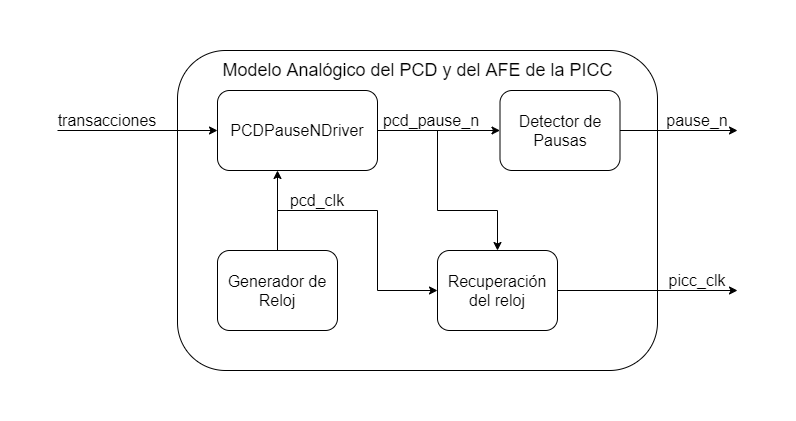
\includegraphics[width=1.0\textwidth]{./img/analogue_model}
  \caption{Modelo del PCD y del AFE de la PICC para uso en simulaciones.}
  \label{fig:analog_model}
\end{figure}

El modelo consiste en cuatro bloques:

\begin{itemize}
  \item Generador de Reloj: Genera un reloj continuo de \SI{13.56}{\mega\hertz} que es un modelo del reloj del PCD.
  \item \textbf{PCDPauseNDriver}: El controlador que envía transacciones mediante pausas. Genera una señal \textit{pcd\_pause\_n} que es la pausa ideal dentro del PCD. La duración de la pausa puede ser elegida por el usuario.
  \item Detector de Pausas: Un modelo del bloque con el mismo nombre en el AFE de la PICC. Genera una señal: \textit{pause\_n} que es una versión retrasada de la señal \textit{pcd\_pause\_n}. Los retardos del flanco ascendente y el flanco descendente pueden ser elegidos por el usuario individualmente.
  \item Recuperación del Reloj: Un modelo del bloque con el mismo nombre en el AFE de la PICC. Genera un reloj basado en lo del PCD, que se detiene durante las pausas. Los retardos entre el comienzo de una pausa y el reloj deteniéndose, y entre el fin de una pausa y el reloj comenzando de nuevo, pueden ser elegidos por el usuario individualmente. Además el usuario puede especificar que el reloj no se detiene, por lo tanto este modelo puede simular el comportamiento de un AFE dónde el reloj es continuo.
\end{itemize}

La \figref{fig:afe_sim} muestra dos simulaciones de una pausa con argumentos de timing diferentes. En el momento de escritura de esta tesis los timings por defectos son basados en simulaciones SPICE del AFE implementado por Alcalde Bessia por otro proceso de fabricación~\cite{fabricio_eamta}. Cuándo exista una implementación del AFE para el proceso de fabricación XFAB XH018 es altamente sugerido que los valores en este modelo sean actualizados para adecuarse la situación real.

\begin{figure}[htb]
  \centering
  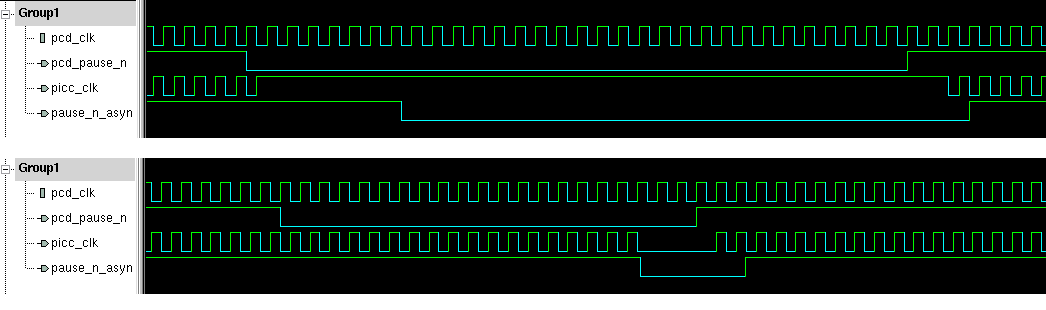
\includegraphics[width=1.0\textwidth]{./img/analogue_sim}
  \caption{Dos ejemplos con timings diferentes del modelo analógico del PCD y el AFE de la PICC.}
  \label{fig:afe_sim}
\end{figure}

% Estructura de los Bancos de Pruebas
\FloatBarrier
\subsection{Estructura de los Bancos de Pruebas}

La mayoría de los módulos en esta tesis son verificados con un banco de prueba que tiene una de las dos estructuras mostrado en la \figref{fig:tb_structures}.

\begin{figure}[htb]
  \centering
  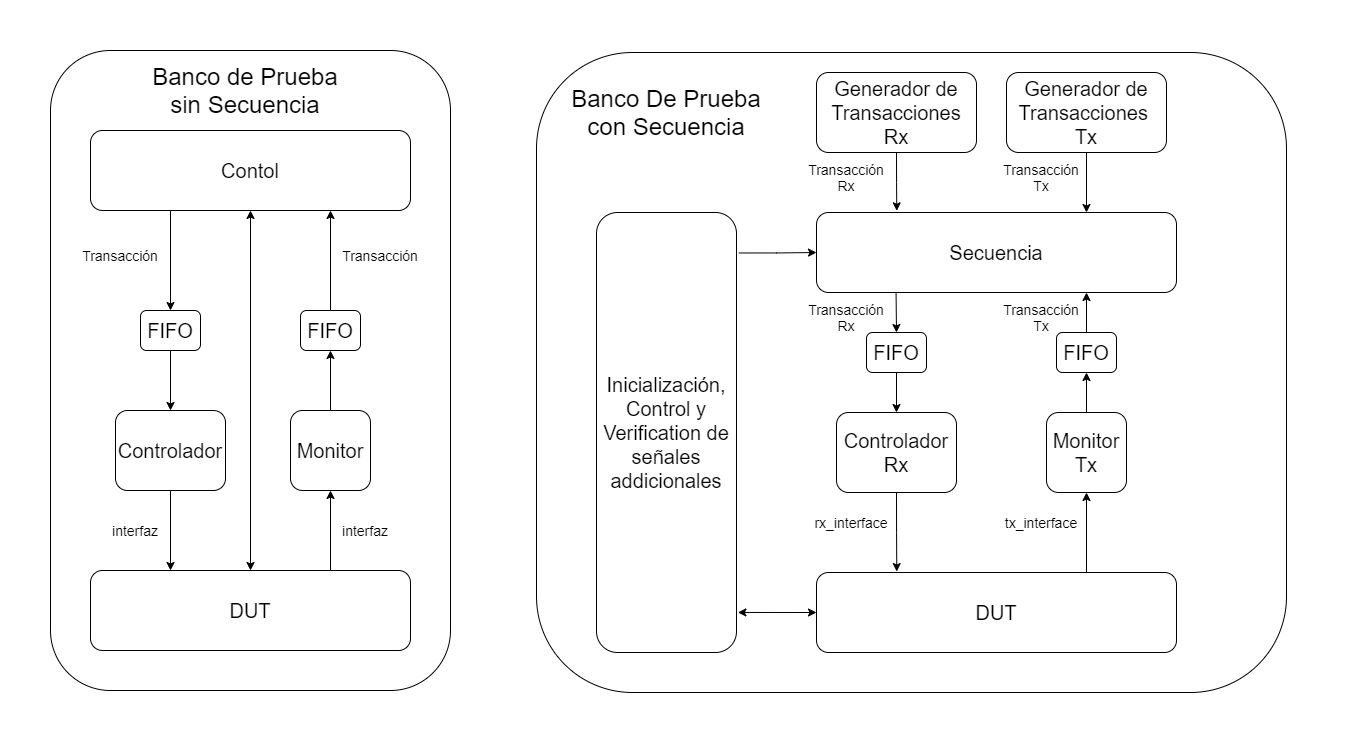
\includegraphics[width=1.0\textwidth]{./img/verification3}
  \caption{Dos estructuras comunes de los bancos de pruebas.}
  \label{fig:tb_structures}
\end{figure}

Los módulos que simplemente reciben tramas, operan sobre ellas, y las reenvían, son verificados con un banco de prueba sin una secuencia (izquierda). El bloque de control genera una transacción en el formato adecuado y la pasa al controlador mediante un FIFO. El DUT la recibe por su interfaz de sumidero, la procesa, y la reenvía sobre su interfaz de fuente. El monitor detecta la trama reenviada, construye una transacción, y la pasa al bloque de control mediante otro FIFO. Finalmente el bloque de control compara esas transacciones para verificar que la trama fue modificada correctamente.

Los módulos que reciben solicitudes del PCD y envían respuestas, son verificados con un banco de prueba que incluye una secuencia (derecha). El banco de prueba define una nueva clase de secuencia que extiende una de las secuencias genéricas, y sustituye varios métodos para implementar funcionamiento específico a ese banco de prueba. Esos bancos de pruebas funcionan de una manera parecida a los bancos de prueba sin secuencias, pero las tramas enviadas son elegidas por las pruebas en la secuencia, y son generadas por el generador de transacciones. Además las respuestas enviadas por el DUT son comparadas en la secuencia con las respuestas esperadas.


% ISO/IEC 14443A núcleo IP
% --------------------------------
\FloatBarrier
\section{ISO/IEC 14443A núcleo IP}

Está parte de la tesis está diseñada para ser una implementación digital genérica de la norma ISO/IEC 14443 para PICCs tipo A. Cuándo se combina con una AFE puede ser usado para cualquier proyecto que requiera funcionar como una PICC tipo A. La implementación  se divide en tres partes principales para las partes dos, tres, y cuatro de la norma.

% ISO/IEC 14443-2A
\FloatBarrier
\subsection{ISO/IEC 14443-2A}

Está parte de la implementación consiste en cinco módulos y sus bancos de pruebas correspondientes. Para la ruta de recepción de tramas hay un solo módulo: \textbf{sequence\_decode}, que convierte una serie de pausas a tramas de bits. La ruta de transmisión consiste en tres módulos que convierten tramas de bits a una señal apta para manejar el modulador de carga. Las módulos son:

\begin{itemize}
  \item \textbf{subcarrier}: Genera la subportadora.
  \item \textbf{bit\_encoder}: Genera la codificación manchester desde una trama de bits.
  \item \textbf{tx}: Recibe la trama a transmitir, agrega el SOC, y produce la salida al modulador de carga mediante los módulos: \textbf{subcarrier} y \textbf{bit\_encode}.
\end{itemize}

Finalmente hay un módulo: \textbf{iso14443\_2a} que es el módulo más alto de esta parte de la norma.

% subcarrier
\FloatBarrier
\subsubsection{subcarrier}

Este módulo genera la señal de la subportadora cuándo pedido. Las entradas y salidas son descritas en el \tabref{tab:ports_subcarrier}. La norma dicta que la subportadora debería tener frecuencia igual a fc/16, y que el periodo de bit debería comenzar con el estado cargado de la portadora [ISO/IEC 14443A]. Esto significa que la salida \textit{subcarrier} es una onda cuadrada que comienza con valor ‘1’, y tiene un periodo de 16 ciclos del reloj.

\begin{table}[htb]
  \centering
  \rowcolors{2}{white}{lightgray!35}
  \begin{tabulary}{\linewidth}{l|l|L}
    \textbf{Nombre}&\textbf{Dirección}&\textbf{Descripción} \\
    \hline
    clk&Entrada&Reloj. \\
    rst\_n&Entrada&Reset activo bajo. \\
    en&Entrada&Señal de activación. \\
    subcarrier&Salida&Subportadora. \\
  \end{tabulary}
  \caption{Entradas y Salidas del módulo \textbf{subcarrirer}.}
  \label{tab:ports_subcarrier}
\end{table}

La implementación consiste en un contador de tres bits, cuándo el módulo no está activado el contador es detenido con valor cero, y la salida \textit{subcarrier} está ‘0’. Cuándo la señal \textit{en} sube a ‘1’, la salida \textit{subcarrier} es asignada a ‘1’ y el contador comienza a contar. Cada ocho ciclos del reloj el contador completa su cuenta, y la salida \textit{subcarrier} invierte su estado lógico.

El banco de prueba consiste en activar el DUT tres veces. La primera vez es activado por 256 ciclos (dos duraciones de bits). La segunda vez es activado por seis ciclos, para que la subportadora es ‘1’ cuando se desactiva el DUT. Finalmente la tercera vez el módulo es activado para trece ciclos, para que la subportadora es ‘0’ cuando se desactiva el DUT. Hay cuatro aserciones que verifican el comportamiento:

\begin{itemize}
  \item La subportadora está ‘0’ mientras el DUT está en reset.
  \item La subportadora está ‘0’ mientras el DUT está desactivado.
  \item Un ciclo después del flanco ascendente de la señal \textit{en} el subcarrier está ‘1’.
  \item Cuando el DUT está activado la subportadora tiene un periodo de 16 ciclos del reloj con un ciclo de trabajo de 50\%.
\end{itemize}

El informe de cobertura da un resultado de 100\% cobertura.

% bit_encoder
\FloatBarrier
\subsubsection{bit\_encoder}

Este módulo es un sumidero por la \textit{tx\_interface}, recibe tramas de bits y las convierte a su codificación Manchester con duración de bit de 128 ciclos del reloj. Las entradas y salidas son descritas en el \tabref{tab:ports_bit_encoder}.

\begin{table}[htb]
  \centering
  \rowcolors{2}{white}{lightgray!35}
  \begin{tabulary}{\linewidth}{l|l|L}
    \textbf{Nombre}&\textbf{Dirección}&\textbf{Descripción} \\
    \hline
    clk&Entrada&Reloj. \\
    rst\_n&Entrada&Reset activo bajo. \\
    en&Entrada&Señal de activación. \\
    in\_iface&Entrada&Sumidero de la, \textit{tx\_interface}. Las tramas a transmitir. \\
    encoded\_data&Salida&Codificación Manchester de cada bit. \\
    last\_tick&Salida&Indica el último ciclo de cada periodo de bit. \\
  \end{tabulary}
  \caption{Entradas y Salidas del módulo \textbf{bit\_encoder}.}
  \label{tab:ports_bit_encoder}
\end{table}

La implementación de este módulo consiste en un contador de siete bits para contar la duración de bit de 128 ciclos. Cuando el módulo no está activado el contador tiene valor cero, y cuando está activado cuenta repetitivamente. Al principio de cada duración de bit, eso es decir cuándo el contador tiene valor cero y el módulo está activado, la salida \textit{encoded\_data} es asignada al valor del bit actual presente en la \textit{in\_iface}. En el medio del periodo del bit, cuando el contador tiene valor 64, la salida \textit{encoded\_data} se invierte. Esto significa que para envíar el bit 0, \textit{encoded\_data} está ‘0’ por 64 ciclos y después ‘1’ por 64 ciclos más. La señal \textit{tx\_interface.req} está pulsada por un ciclo del reloj en el medio del periodo de bit, para pedir que la fuente prepare el siguiente bit. Finalmente la salida \textit{last\_tick} está pulsada cuándo el contador tiene valor 127, esta salida es usada para determinar cuándo desactivar este módulo después del último bit de la trama.

El banco de prueba tiene un \textbf{TxBitIfaceSourceDriver} para envíar tramas al DUT. No utiliza un monitor, ya que es el único módulo que genera una salida en este formato. Antes de envíar cada trama, la transacción es convertida a una cola que consiste en los valores esperados por cada ciclo de la trama. Una aserción verifica que la salida \textit{encoded\_data} del DUT corresponde con esa cola. Las pruebas consisten en:

\begin{itemize}
  \item Enviar dos transacciones de un solo bit cada una, con valores ‘0’ y ‘1’.
  \item Enviar dos transacciones de dos bit cada una, con valores “00” y “10”.
  \item Enviar mil transacciones de data y tamaño aleatorios.
\end{itemize}

Las aserciones son:

\begin{itemize}
  \item Cuándo el DUT está en reset o no está activado, las salidas: \textit{in\_iface.req} y \textit{last\_tick} están ‘0’s.
  \item La salida \textit{last\_tick} solo está ‘1’ para un ciclo del reloj a la vez.
  \item Mientras el DUT está activado, las salidas \textit{in\_iface.req} y \textit{last\_tick} pulsan por un ciclo del reloj, cada 128 ciclos.
  \item Después del flanco ascendente de la entrada \textit{en}, la salida \textit{last\_tick} está ‘0’ por 127 ciclos del reloj y ‘1’ en el siguiente ciclo.
\end{itemize}

El informe de cobertura da un resultado de 100\% por el DUT.

% tx
\FloatBarrier
\subsubsection{tx}

El módulo \textbf{tx} instancia los módulos: \textbf{subcarrier} y \textbf{bit\_encoder}, e incluye una máquina de estados sencilla que: agrega el SOC a las tramas, activa los submódulos, y manejar la señal \textit{tx\_interface.req} para pedir que la fuente prepare el siguiente bit. Finalmente la señal \textit{lm\_out} es el AND lógico de la subportadora y la señal \textit{encoded\_data}, esta salida es registrada para prevenir glitches llegando al modulador de carga. Las entradas y salidas son descritas en el \tabref{tab:ports_tx}.

\begin{table}[htb]
  \centering
  \rowcolors{2}{white}{lightgray!35}
  \begin{tabulary}{\linewidth}{l|l|L}
    \textbf{Nombre}&\textbf{Dirección}&\textbf{Descripción} \\
    \hline
    clk&Entrada&Reloj. \\
    rst\_n&Entrada&Reset activo bajo. \\
    in\_iface&Entrada&Sumidero de la \textit{tx\_interface}. \\
    lm\_out&Salida&Señal hacia el modulador de carga. \\
  \end{tabulary}
  \caption{Entradas y Salidas del módulo \textbf{tx}.}
  \label{tab:ports_tx}
\end{table}


El banco de prueba tiene un controlador \textbf{TxBitIfaceSourceDriver} y un monitor \textbf{LoadModulatorMonitor}. Las pruebas son:

\begin{itemize}
  \item El SOC es agregado correctamente. Esto es hecho en el monitor, que verifica que todas las tramas comienzan con un SOC.
  \item La salida \textit{lm\_out} está en ‘0’ cuándo la fuente no está enviando una trama.
  \item Tramas son enviadas correctamente. Cien transacciones aleatorias son enviadas y las transacciones detectadas por el monitor son comparadas a las enviadas dentro de una aserción.
\end{itemize}

El informe de cobertura da un resultado de 92\% por el DUT. Las partes que faltan cobertura no son relevantes, por ejemplo no hay una transición desde el estado State\_SOC al estado State\_IDLE, ya que no está permitido transmitir una trama SOC aislada.

% sequence_decode
\FloatBarrier
\subsubsection{sequence\_decode}
\label{sec:sequence_decode}

El módulo \textbf{sequence\_decode} convierte series de pausas a tramas de bits, y las envía al siguiente módulo mediante una fuente de la \textit{rx\_interface}. La norma ISO/IEC 14443-2 [iso/iec 14443-2] especifica que la duración de bit por recepción es 128 ciclos de la portadora. La existencia de una pausa dentro de una duración de bit y su ubicación determina qué tipo de secuencia es: X, Y o Z. Una pausa al principio de la duración de bit es una secuencia Z, una pausa en el medio de la duración de bit es una secuencia X, y una duración de bit sin pausas es una secuencia Y.  La \figref{fig:sequences} muestra estas secuencias. Cada trama comienza con una secuencia Z (SOC). Un ‘1’ es transmitido con una secuencia X. La secuencia usada para transmitir un ‘0’ depende en la última secuencia. Una secuencia Y es usada cuando la última secuencia fue una X, y una secuencia Z es usada en otros casos. Cada trama termina con un EOC, que es transmitido con un ‘0’ lógico seguido por la secuencia Y. Finalmente una secuencia X seguida por una secuencia Z no es permitido y debería estar contado como un error.

En teoría el proceso de convertir una serie de pausas a secuencias es: contar el número de ciclos del reloj en cada duración de bit para determinar dónde comienza la pausa. En la práctica es más complicado debido a que el reloj puede detenerse durante las pausas. Además el tiempo que el reloj está detenido depende de la implementación del bloque de la recuperación del reloj del AFE, y las propiedades del PCD. Debido a que este núcleo IP está diseñado para ser genérico, tiene que funcionar con diferentes AFEs y diferentes PCDs, por lo tanto este módulo fue implementado para funcionar con un amplio rango de comportamientos de relojes. La estrategia propuesta para el módulo \textbf{sequence\_decode} consiste en contar ciclos de clock entre flancos ascendentes de la señal \textit{pause\_n}. Luego a partir del valor de la cuenta se infiere la secuencia recibida. A continuación se analizan las condiciones para aplicar este método de decodificación.

La \figref{fig:rx_timings_tz2z} muestra dos secuencias Z consecutivas. \textit{PCD CLK} y \textit{PICC CLK} son los relojes en el PCD y la PICC respectivamente, \textit{pcd\_pause\_n} es la pausa digital que el PCD transmite, \textit{picc\_pause\_n} es la pausa detectada en el AFE, \textit{PICC CLK ACTIVE} indica cuándo el reloj de la PICC está activo. El tiempo entre los dos flancos ascendentes de las pausas medido en ciclos del reloj del PCD es $T_b = 128$. Si el reloj de la PICC se detiene por $T_{nc}$ ciclos durante las pausas, la PICC mediría $T_{z2z} = T_b - T_{nc}$ ciclos entre los flancos ascendentes de las pausas.

\begin{figure}[htb]
  \centering
  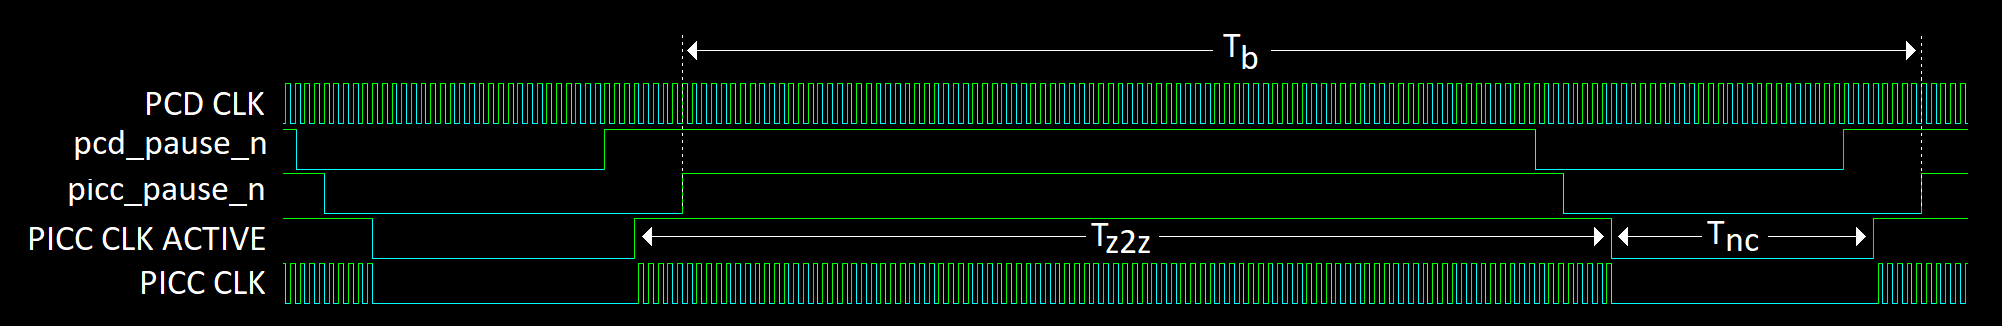
\includegraphics[width=1.0\textwidth]{./img/rx_timings_tz2z}
  \caption{Diagrama de timing de dos pausas y el comportamiento del reloj de la PICC.}
  \label{fig:rx_timings_tz2z}
\end{figure}

La \figref{fig:rx_timings} muestra el número de ciclos entre dos pausas para todas las combinaciones de secuencias posibles. Usa la misma convención de la \figref{fig:rx_timings_tz2z}, $T_{z2x}$ por ejemplo representa la cantidad de ciclos que la PICC mide entre los flancos ascendentes de las pausas cuándo el PCD transmite una secuencia Z seguida por una secuencia X. Esta convención sigue válida aun cuándo el AFE produce un reloj continuo, y por lo tanto $T_{nc}$ = 0.

\begin{figure}[htb]
  \centering
  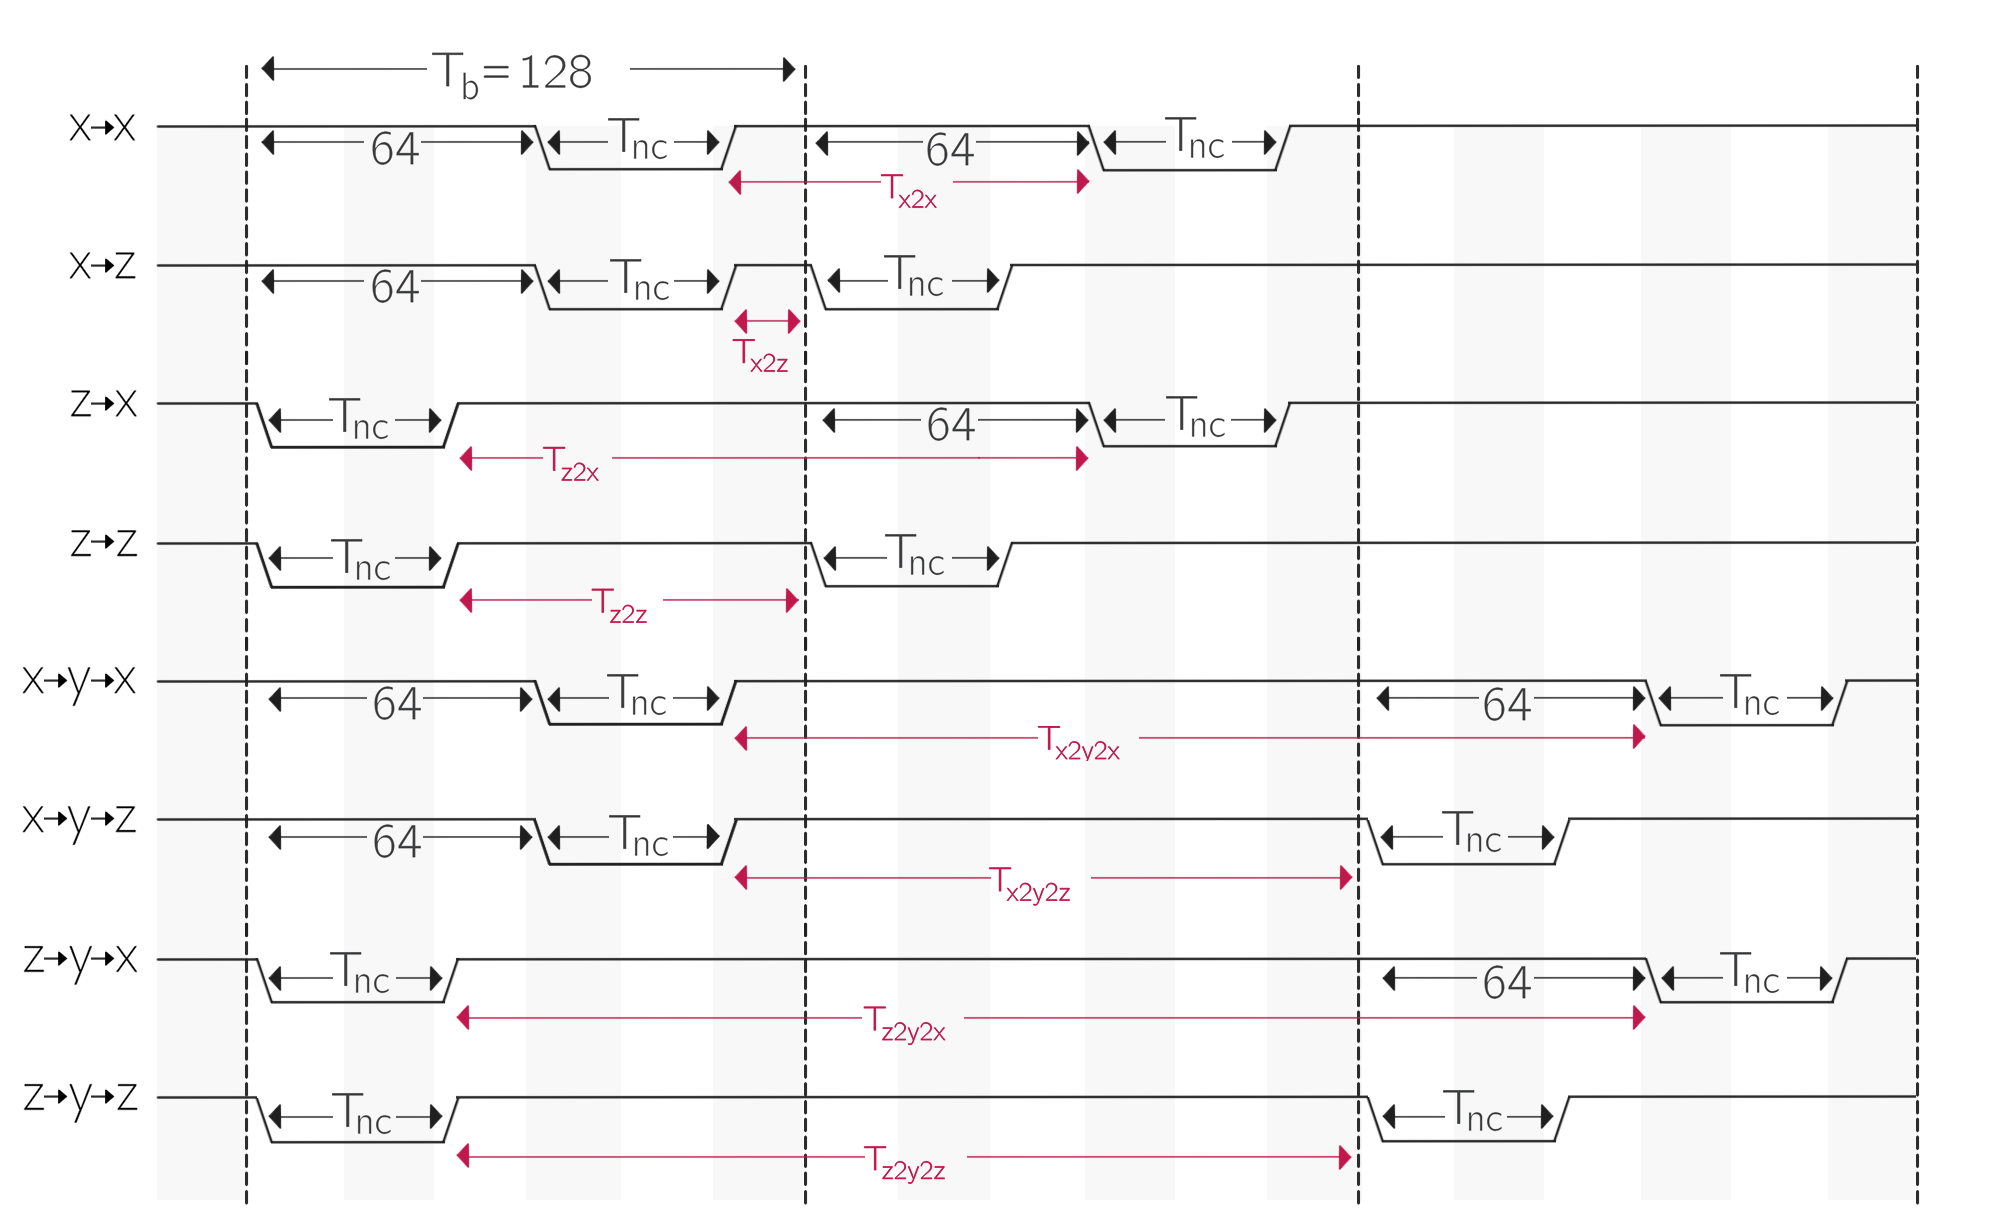
\includegraphics[width=1.0\textwidth]{./img/rx_timings}
  \caption{Números de ciclos posibles entre dos pausas.}
  \label{fig:rx_timings}
\end{figure}
\message{TODO: Update this image}

Se define $T_{nc\_min}$ y $T_{nc\_max}$ como el número de ciclos mínimos y máximos que el reloj puede estar detenido para que las secuencias puedan ser decodificadas correctamente. Este análisis es necesario para considerar variaciones en el comportamiento de los PCDs y los AFEs. Considerando las combinación de secuencias: Z~$\rightarrow$~Z, y Z~$\rightarrow$~X y observando la \figref{fig:rx_timings}, se puede calcular:

\begin{align*}
    T_{z2z\_max} &= 128 - T_{nc\_min} \\
    T_{z2x\_min} &= 192 - T_{nc\_max} \\
\end{align*}

Conociendo que $T_{z2x\_min} > T_{z2z\_max}$, para que se pueda distinguir entre una Z~$\rightarrow$~X y una Z~$\rightarrow$~Z, se puede derivar:

\begin{align*}
    192 - T_{nc\_max} &> 128 - T_{nc\_min} \\
    T_{nc\_max} &< T_{nc\_min} + 64 \\
\end{align*}

Para soportar AFEs que usan un PLL para proveer un reloj continuo, debería aceptarse $T_{nc\_min}$ igual a 0. Además es posible que haya jitter en la detección de los flancos ascendentes de las las pausas en el AFE. Ese jitter puede causar que una PICC cuente un número de ciclos ligeramente diferente entre dos secuencias cada vez que ocurren. Ese comportamiento es igual a si el jitter fue en el número de ciclos que el reloj está detenido. En esta implementación es requerido que ese jitter es a lo máximo tres ciclos, por lo tanto se usa un $T_{nc\_min} = -3$, lo que da un $T_{nc\_max} < 61$.

Considerando el caso de una secuencia X seguido por una secuencia Y se requiere que: $T_{x2y\_min} > T_{x2x\_max}$, es decir que después de una secuencia X, el momento que este módulo emite una secuencia Y tiene que ser después del último momento que puede llegar una pausa que indicaría otra secuencia X. Por lo tanto:

\begin{align*}
    T_{x2y\_min} &> 128 - T_{nc\_min} \\
    T_{x2y\_min} &> 131 \\
\end{align*}

Eligiendo $T_{x2y\_min} = 132$, significa que si no hay una pausa detectada por más de 131 ciclos después de una secuencia X, se asume el arribo de una secuencia Y. Finalmente considerando el serie de secuencias: X~$\rightarrow$~Y~$\rightarrow$~Z:

\begin{align*}
    T_{x2y2z\_min} &= 192 - T_{nc\_max} \\
               &= T_{x2y\_min} + T_{y2z\_min} \\
               &= 132 + T_{y2z\_min} \\
    \\
    192 - T_{nc\_max} &= 132 + T_{y2z\_min} \\
    T_{y2z\_min} &= 60 - T_{nc\_max} \\
\end{align*}

Una $T_{y2z\_min} = 0$, implica que la secuencia Y puede ser detectada en el mismo ciclo de un flanco ascendente de una pausa por una secuencia Z. Para simplificar el diseño esto no se permite, así:

\begin{align*}
    T_{y2z\_min} &> 0 \\
    60 - T_{nc\_max} &> 0 \\
    T_{nc\_max} &< 60 \\
\end{align*}

En resumen es posible diseñar un sistema que decodifica una serie de pausas a secuencias, siempre que el AFE pueda garantizar que el reloj nunca se detiene por más de 59 ciclos. Para soportar hasta tres ciclos de jitter en la detección de las pausas como especificado arriba es recomendado que el reloj no se detenga por más de 56 ciclos. El mismo diseño va a funcionar con un AFE que produce un reloj continuo. Estos requisitos por el AFE son razonables, debido a que la duración de pausa máxima determinada con la \figref{fig:pause} y el \tabref{tab:pause_values} es 56,5 ciclos del reloj, medido entre los puntos 1 y 2, dónde él amplitud de la portadora es a 90\% de su original.

Usando $T_{nc\_min} = -3$, y $T_{nc\_max = 59}$, es posible diseñar un sistema que decodifica pausas a secuencias, dependiendo de la última secuencia detectada y el número de ciclos contados entre los flancos ascendentes de las pausas. La decodificación usada es mostrada en la\tabref{tab:sequence_decode_timings}. Valores fuera de estos rangos son considerados errores.

\begin{table}[htb]
  \centering
  \begin{tabular}{c|r|r|c}
    \rowcolor{lightgray!35}
    \textbf{Última Secuencia} & \textbf{Mín Ciclos} & \textbf{Máx Ciclos} & \textbf{Proxima Secuencia} \\
    \hline
                        & 69             & 131   & X \\
    \multirow{-2}{*}{X} & 132 (timeout)  & -     & Y \\
    \rowcolor{lightgray!35}
                        & 69             & 131   & Z \\
    \rowcolor{lightgray!35}
                        & 132            & 195   & X \\
    \rowcolor{lightgray!35}
    \multirow{-3}{*}{Z} & 196 (timeout)  & -     & Y \\
                        & 1              & 64    & Z \\
                        & 65             & 127   & X \\
    \multirow{-3}{*}{Y} & 128 (timeout)  & -     & Y \\
  \end{tabular}
  \caption{Decodificación de pausas basado en la última secuencia y el tiempo entre pausas.}
  \label{tab:sequence_decode_timings}
\end{table}

La \tabref{tab:ports_sequence_decode} muestra las entradas y salidas de este módulo. La implementación consiste en dos partes. La primera parte determina la secuencia desde las pausas detectadas. El diseño comienza en un estado inactivo, cuándo detecta la primera pausa emite una secuencia Z debido a que el SOC de la trama es una secuencia Z. Después emite secuencias cuándo pausas están detectadas o cuándo timeouts ocurren usando el método descrito arriba. Después de detectar dos secuencias Y consecutivas, eso es dos duraciones de bits sin pausas, se vuelve al estado inactivo, y espera por la próxima trama. En el caso de detectar un error, no emite más secuencias y después de haber detectado tres duraciones de bits sin pausas vuelve al estado inactivo. La segunda parte de este módulo decodifica las secuencias a una trama de bits y lo envía sobre la \textit{out\_iface} para el posterior procesamiento en otros módulos.

\begin{table}[htb]
  \centering
  \rowcolors{2}{white}{lightgray!35}
  \begin{tabulary}{\linewidth}{l|l|L}
    \textbf{Nombre}&\textbf{Dirección}&\textbf{Descripción} \\
    \hline
    clk&Entrada&Reloj. \\
    rst\_n&Entrada&Reset activo bajo. \\
    pause\_n\_synchronised &Entrada&Pausa, activa baja, sincronizada.\\
    out\_iface&Salida&Fuente de la \textit{rx\_interface}.\\
  \end{tabulary}
  \caption{Entradas y Salidas del módulo \textbf{sequence\_decode}.}
  \label{tab:ports_sequence_decode}
\end{table}

Para verificar este módulo el banco de prueba envía varias transacciones mediante el controlador \textbf{PCDPauseNDriver} en el modelo del AFE, que maneja la entrada del DUT \textit{pause\_n\_synchronised}. El monitor \textbf{RxBitIfaceMonitor}, monitoriza la salida \textit{out\_iface} y emite transacciones por las tramas detectadas. Esas transacciones son comparadas con las enviadas para verificar que el DUT decodifica correctamente las pausas. Las transacciones enviadas son:

\begin{itemize}
  \item La transacción ZZXXYZXYXYY, y la transacción ZXYZY. Estas dos transacciones verifican todas las filas en el \tabref{tab:sequence_decode_timings}.
  \item Cincuenta transacciones aleatorias sin errores.
  \item La transacción: ZXZZXYXYY para verificar que la transición Z -> X es detectada como un error, y que secuencias después del error son ignoradas.
\end{itemize}

Estas pruebas son repetidas varias veces con diferentes timings configurados en el modelo del AFE. Los parámetros de timings son:

\begin{itemize}
  \item La duración de la pausa.
  \item Si el reloj se detiene durante las pausas o no.
  \item El retardo entre el principio de una pausa enviada por el PCD y el reloj deteniéndose.
  \item El retardo entre el final de una pausa enviada por el PCD y el reloj activándose de nuevo.
  \item El retardo entre el principio de una pausa enviada por el PCD y el AFE detectándolo.
  \item El retardo entre el final de una pausa enviada por el PCD y el AFE detectándolo.
\end{itemize}

Para asegurar que un amplio rango de las condiciones posibles son verificadas estos tiempos son elegidos aleatoriamente con restricciones sobre cuántos flancos el reloj de la PICC pueden faltar comparado al reloj del PCD. El código que elige esos valores toma un argumento \textit{missing\_edges} que define el número de flancos que faltan al reloj de la PICC. Este argumento es usado con la sintaxis de SystemVerilog “std::randomize() with {}” que permite especificar una lista de variables a randomizar y una lista de condiciones que los resultados deben cumplir. Antes fue especificado que este diseño funciona si el reloj se detiene cómo mínimo 0 ciclos, y cómo máximo 59 ciclos. Esos valores corresponden con un \textit{missing\_edges} entre 0 y 118. Las pruebas son repetidos cien veces para cada uno de \textit{missing\_edge} igual a  0 a 3 y 115 a 118, y después mil veces con \textit{missing\_edges} elegido aleatoriamente entre 4 y 114.

El informe de cobertura da un resultado de 95\% por el DUT. Los tres sitios en los que falta cobertura son condiciones imposibles de ocurrir, por ejemplo emitiendo una secuencia Z después de una secuencia X. La norma define una Z~$\rightarrow$~X como un error, por lo tanto cuando el DUT detecta la Z emite un error mediante \textit{out\_iface.error}, en vez de tratarla como una secuencia Z normal.

% iso14443_2a
\FloatBarrier
\subsubsection{iso14443\_2a}

Este módulo simplemente instancia los módulos: \textbf{tx} y \textbf{sequence\_decode} como se muestra la \figref{fig:iso14443_2a}. Las entradas y salidas son descritas en el \tabref{tab:ports_iso14443_2a}.

\begin{table}[htb]
  \centering
  \rowcolors{2}{white}{lightgray!35}
  \begin{tabulary}{\linewidth}{l|l|L}
    \textbf{Nombre}&\textbf{Dirección}&\textbf{Descripción} \\
    \hline
    clk&Entrada&Reloj. \\
    rst\_n&Entrada&Reset activo bajo. \\
    pause\_n\_synchronised &Entrada&Pausa, activa baja, sincronizada. \\
    rx\_iface&Salida&Fuente de la \textit{rx\_interface}. \\
    tx\_iface&Entrada&Sumidero de la \textit{tx\_interface}. \\
    lm\_out&Salida&Señal hacia el modulador de carga. \\
  \end{tabulary}
  \caption{Entradas y Salidas del módulo \textbf{iso14443\_2a}.}
  \label{tab:ports_iso14443_2a}
\end{table}

\begin{figure}[htb]
  \centering
  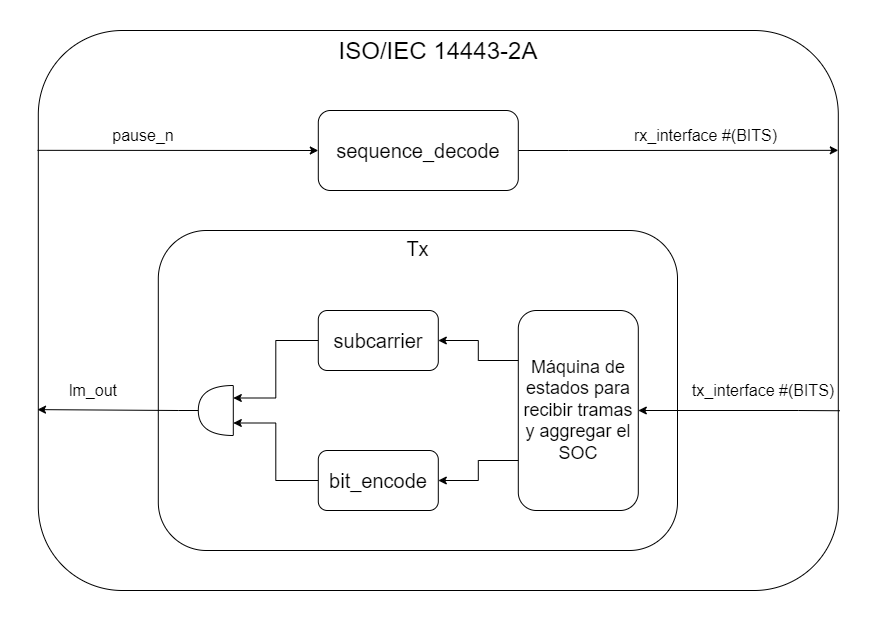
\includegraphics[width=0.8\textwidth]{./img/iso14443_2a.drawio}
  \caption{Diagrama en bloque del módulo \textbf{iso14443\_2a}.}
  \label{fig:iso14443_2a}
\end{figure}

El banco de prueba funciona de forma loopback, genera mil transacciones aleatoriamente, que son transmitidos mediante el controlador \textbf{PCDPauseNDriver} en el modelo del AFE. El monitor \textbf{RxBitIfaceMonitor} recibe las tramas procesadas por el DUT sobre la \textit{rx\_iface}. Cada transacción recibida por el monitor es convertida a una \textbf{TxBitTransaction} y es reenviado sobre la \textit{tx\_iface} con un controlador \textbf{TxBitIfaceSourceDriver}. Finalmente un monitor \textbf{LoadModulatorMonitor} detecta las tramas transmitidas por el DUT sobre su salida \textit{lm\_out}. Cada transacción recibida por ese monitor es comparada con las transacciones enviadas en una aserción. La \figref{fig:iso14443_2a_tb} muestra un diagrama en bloques del banco de prueba.

\begin{figure}[htb]
  \centering
  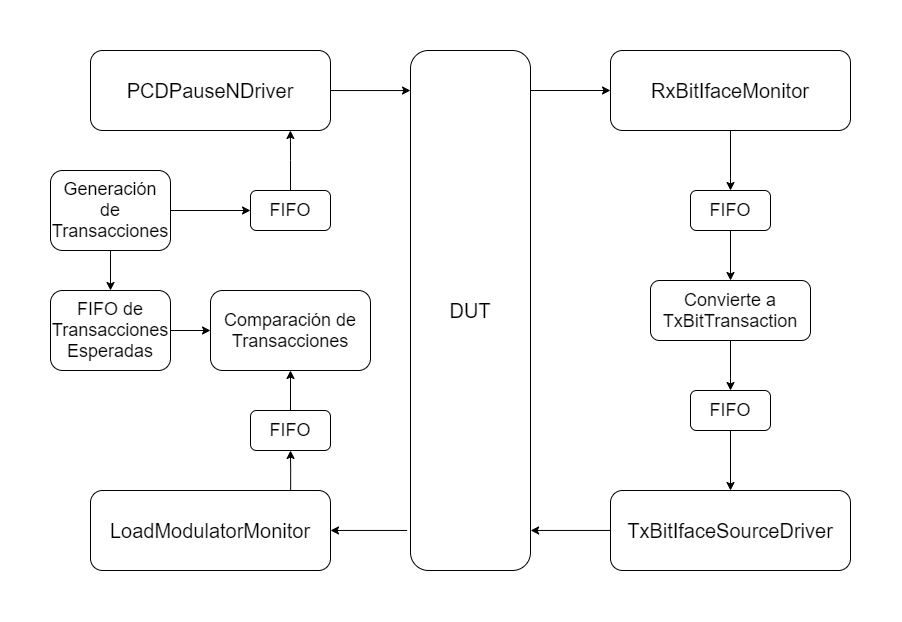
\includegraphics[width=0.9\textwidth]{./img/iso14443_2a_tb.drawio}
  \caption{Diagrama en bloques del banco de prueba para el módulo \textbf{iso14443\_2a}}
  \label{fig:iso14443_2a_tb}
\end{figure}

Debido a que este módulo solo consiste en la instanciación de dos módulos, la única métrica de cobertura generada por el DUT, no incluyendo los submódulos auxiliares, es de cambio de estado de las señales y compuertas (toggle), que tiene 100\% cobertura.

% ISO/IEC 14443-3A
\FloatBarrier
\subsection{ISO/IEC 14443-3A}

Esta parte de la implementación consiste en once módulos y sus bancos de pruebas correspondientes. 

\begin{itemize}
  \item \textbf{frame\_decode}: Verifica y quita los bits de paridad de tramas recibidas desde el PCD.
  \item \textbf{desreialiser}: Convierte una trama de bits a una trama de bytes. Usado en la ruta de recepción.
  \item \textbf{FDT}: Genera una señal para activar la transmisión de una respuesta, para que se cumpla con el FDT definido en la norma.
  \item \textbf{CRC\_A}: Calcula el CRC16 de una serie de bits.
  \item \textbf{crc\_control}: Verifica el CRC16 de tramas recibidas, y genera el CRC16 de tramas a transmitir.
  \item \textbf{serialiser}: Convierte una trama de bytes a una trama de bits. Usado en la ruta de transmisión.
  \item \textbf{frame\_encode}: Comienza la transmisión de una trama al PCD cuándo recibe la señal de activación del módulo FDT, y agrega los bits de paridad y el CRC16 a la trama.
  \item \textbf{framing}: Instancia los módulos de arriba.
  \item \textbf{initialisation}: Recibe tramas de inicialización y anticolisión desde el PCD, actúa sobre ellas, y responde con la respuesta adecuada.
  \item \textbf{routing}: Rutea tramas recibidas desde el PCD al módulo apto para procesarlas, y rutea las respuestas desde ese módulo para transmitir al PCD. El ruteo es controlado basado en el estado actual de la PICC.
  \item \textbf{iso14443\_3a}: El módulo más alto para esta parte de la norma, instancia los módulos: \textbf{framing}, \textbf{initialisation} y \textbf{routing}.
\end{itemize}

% frame_decode
\FloatBarrier
\subsubsection{frame\_decode}

Este módulo tiene un sumidero de la \textit{rx\_interface} que está conectado a la fuente del módulo \textbf{iso14443\_2a}, y una fuente, también de la \textit{rx\_interface} que está conectado al próximo módulo. Las Tramas son recibidas en una serie de bits, después de cada 8 bits hay un bit de paridad. Esos bits de paridad son verificados y quitados antes de reenviar la trama por la fuente. Las entradas y salidas son descritas en el \tabref{tab:ports_frame_decode}.

\begin{table}[htb]
  \centering
  \rowcolors{2}{white}{lightgray!35}
  \begin{tabulary}{\linewidth}{l|l|L}
    \textbf{Nombre}&\textbf{Dirección}&\textbf{Descripción} \\
    \hline
    clk&Entrada&Reloj. \\
    rst\_n&Entrada&Reset activo bajo. \\
    in\_iface&Entrada&Sumidero de la \textit{rx\_interface}. \\
    out\_iface&Salida&Fuente de la \textit{rx\_interface}. \\
    last\_bit&Salida&Último bit recibido. \\
  \end{tabulary}
  \caption{Entradas y Salidas del módulo \textbf{frame\_decode}.}
  \label{tab:ports_frame_decode}
\end{table}

El tipo de paridad definido por la norma es impar, eso es a decir que el número de unos en el byte más el bit de paridad debería ser impar. Por ejemplo el byte: 8’b0101\_1100, tiene cuatro ‘1’s, cuatro es par, así el bit de paridad debe ser ‘1’, para que el total de los ‘1’s sea impar.

Los bits de paridad son verificados y quitados mediante el siguiente proceso. Al principio de cada trama, un indicador \textit{expected\_parity} es inicializado a ‘1’. Después cuándo cada uno de los primeros ochos bits son recibidos, son reenviados, y ese indicador es actualizado con el resultado de: \textit{expecetd\_parity} XOR \textit{in\_iface.data}. Ese cálculo invierte el valor de \textit{expected\_parity} cada vez que un ‘1’ es recibido. El noveno bit es el bit de paridad, así es comparado con \textit{expected\_parity} para verificar que es correcto. Este proceso se repite hasta el fin de la trama, o hasta un error es detectado. 

Hay tres errores que pueden ser detectados en este módulo: Un error indicado en la \textit{in\_iface}, Un error en un bit de paridad, y una trama que le falta su último bit de paridad. Para soportar tramas cortas y de anticolisiones que pueden terminar con un byte parcial sin un bit de paridad, ese último error solo es emitido si una trama termina con un byte entero.

Finalmente la salida \textit{last\_bit} indica el último bit recibido, incluyendo bits de paridad. Esta señal es usada en el módulo \textbf{FDT} para determinar cuándo comenzar a enviar la respuesta.

El banco de prueba para este módulo consiste en un controlador \textbf{RxBitIfaceDriver} y un monitor \textbf{RxBitIfaceMonitor}. Por cada prueba una transacción es generada aleatoriamente, los bits de paridad son agregados, es enviada por el controlador, el resultado es recibido por el monitor y es comparado con la transacción enviada. Las pruebas son:

\begin{itemize}
  \item Enviar una transacción de 8 bits más el bit de paridad correcto.
  \item Enviar una transacción de 8 bits más el bit de paridad equivocado.
  \item Enviar una transacción de 8 bits que falta el bit de paridad.
  \item Enviar mil transacciones de 8 bits cada uno, con un error enviado por el controlador.
  \item Enviar ocho transacciones con cero a siete bits en orden.
  \item Envíar mil transacciones cada uno con un número de bits aleatorio entre uno y ochenta, más los bits de paridad correctos.
  \item Envíar mil transacciones cada uno con un número de bits aleatorio entre ocho y ochenta, con un bit de paridad equivocado y los demás correctos.
  \item Enviar mil transacciones con un número de bytes entero entre 1 y diez, más los bits de paridad por cada byte menos el último.
\end{itemize}

Hay dos aserciones concurrentes para verificar que la señal \textit{last\_bit} es correcta. La primera confirma que la señal corresponde con la última bit enviada. La segunda verifica que esa señal no cambia entre tramas.

El informe de cobertura da el DUT un resultado de 100\%.

% deserialiser
\FloatBarrier
\subsubsection{deserialiser}

% FDT
\FloatBarrier
\subsubsection{FDT}

% CRC_A
\FloatBarrier
\subsubsection{CRC\_A}

% crc_control
\FloatBarrier
\subsubsection{crc\_control}

% serialiser
\FloatBarrier
\subsubsection{serialiser}

% frame_encode
\FloatBarrier
\subsubsection{frame\_encode}

% framing
\FloatBarrier
\subsubsection{framing}

% routing
\FloatBarrier
\subsubsection{routing}

% initialisation
\FloatBarrier
\subsubsection{initialisation}

% ISO/IEC 14443-3A
\FloatBarrier
\subsubsection{ISO/IEC 14443-3A}

% ISO/IEC 14443-4A
\FloatBarrier
\subsection{ISO/IEC 14443-4A}

% ISO/IEC 14443A
\FloatBarrier
\subsection{ISO/IEC 14443A}

% Otros
\FloatBarrier
\subsection{Otros}

% synchroniser
\FloatBarrier
\subsubsection{synchroniser}

% active_low_reset_synchroniser
\FloatBarrier
\subsubsection{active\_low\_reset\_synchroniser}

% pause_n_latch_and_synchroniser
\FloatBarrier
\subsubsection{pause\_n\_latch\_and\_synchroniser}

% Aplicación - Interfaz con el sensor MOSFET de radiación y el ADC
% --------------------------------
\FloatBarrier
\section{Aplicación - Interfaz con el sensor MOSFET de radiación y el ADC}

% Sincronización
\FloatBarrier
\subsection{Sincronización}

% Protocolo
\FloatBarrier
\subsection{Protocolo}

% Ejemplos
\FloatBarrier
\subsection{Ejemplos}

% Marco de Verificación Extendido
\FloatBarrier
\subsection{Marco de Verificación Extendido}

% Implementación
\FloatBarrier
\subsection{Implementación}

% signal_control
\FloatBarrier
\subsubsection{signal\_control}

% adapter
\FloatBarrier
\subsubsection{adapter}

% radiation_sensor_digital_top
\FloatBarrier
\subsubsection{radiation\_sensor\_digital\_top}

% ---------------------------------------------
% Síntesis y Place & Route
% ---------------------------------------------

\FloatBarrier
\chapter{Síntesis y Place \& Route}

% Síntesis
% --------------------------------
\FloatBarrier
\section{Síntesis}

% Preparación de librerías
% --------------------------------
\FloatBarrier
\section{Preparación de librerías}

% Design Planning
% --------------------------------
\FloatBarrier
\section{Design Planning}

% Place & Route
% --------------------------------
\FloatBarrier
\section{Place \& Route}

% LVS / DRC
% --------------------------------
\FloatBarrier
\section{LVS / DRC}

% ---------------------------------------------
% Resultados y Conclusiones
% ---------------------------------------------

\FloatBarrier
\chapter{Resultados y Conclusiones}

% Recomendaciones para Trabajos Futuros
% --------------------------------
\FloatBarrier
\section{Recomendaciones para Trabajos Futuros}

% ---------------------------------------------
% Bibliography
% ---------------------------------------------

\FloatBarrier
\newpage

% Prevent overful hbox warning due to long titles
\emergencystretch=1em
\printbibliography

\end{document}
